\documentclass[final,5p,times]{elsarticle}

\usepackage{amssymb}
\usepackage{amsmath}
\usepackage{booktabs}
\usepackage{graphicx}
\usepackage{microtype}
\usepackage{orcidlink}
\usepackage{xurl}
\usepackage{placeins}
\usepackage{array}
\usepackage{hyperref}

\hypersetup{
    colorlinks=true,
    linkcolor=blue,
    filecolor=magenta,      
    urlcolor=cyan,
    citecolor=blue,
}

\pdfstringdefDisableCommands{%
  \def\orcidlink#1{}%
  \def\corref#1{}%
}

%% ============================================================
%% Versioning and Revision Markup Configuration
%% ============================================================
%% Toggle yellow marker highlights on/off:
%% Set \showdiffsfalse to highlight additions/revisions in yellow marker.
%% Set \showdiffsfalse to compile a clean final manuscript.
%% ============================================================

\newif\ifshowdiffs
\showdiffsfalse

\ifshowdiffs
  \RequirePackage{color,soul}
  \RequirePackage[normalem]{ulem}

  % Highlight color (standard yellow marker)
  \sethlcolor{yellow}

  % Register LaTeX citation and reference macros so \hl won't break on them
  \soulregister\cite7
  \soulregister\citet7
  \soulregister\citep7
  \soulregister\citeauthor7
  \soulregister\citeyear7
  \soulregister\ref7
  \soulregister\eqref7
  \soulregister\pageref7
  \soulregister\autoref7
  \soulregister\url7

  % Revision markup commands
  \DeclareRobustCommand{\revised}[1]{{\protect\hl{#1}}}
  \DeclareRobustCommand{\added}[1]{{\protect\hl{#1}}}
  \DeclareRobustCommand{\deleted}[1]{{\color{red}\sout{#1}}}
  \DeclareRobustCommand{\replaced}[2]{{\color{red}\sout{#2}}{\protect\hl{#1}}}
\else
  % Clean output: show revised/added text normally, hide deleted text
  \DeclareRobustCommand{\revised}[1]{#1}
  \DeclareRobustCommand{\added}[1]{#1}
  \DeclareRobustCommand{\deleted}[1]{}
  \DeclareRobustCommand{\replaced}[2]{#1}
\fi

% Protect PDF bookmarks and table of contents when hyperref is active
\AtBeginDocument{%
  \pdfstringdefDisableCommands{%
    \def\revised#1{#1}%
    \def\added#1{#1}%
    \def\deleted#1{}%
    \def\replaced#1#2{#1}%
    \def\hl#1{#1}%
  }%
}


\setcounter{topnumber}{5}
\setcounter{bottomnumber}{5}
\setcounter{totalnumber}{10}
\setcounter{dbltopnumber}{5}
\renewcommand{\topfraction}{0.99}
\renewcommand{\bottomfraction}{0.99}
\renewcommand{\textfraction}{0.01}
\renewcommand{\floatpagefraction}{0.7}
\renewcommand{\dbltopfraction}{0.99}
\renewcommand{\dblfloatpagefraction}{0.7}

\journal{SoftwareX}

\begin{document}

\begin{frontmatter}

\title{Wood Surface Defect Detection Under Severe Long-Tail Imbalance: A Comparative Benchmark of Cascade R-CNN, YOLO26, and RF-DETR}

\author[1]{Ricardo Mauricio Chambilla Perca\orcidlink{0009-0002-4863-0637}}
\ead{rchambillap@unsa.edu.pe}

\author[1]{Mariel Alison Jara Mamani\orcidlink{0009-0000-9069-5800}}
\ead{mjarama@unsa.edu.pe}

\author[1]{Christian Raul Mestas Zegarra\orcidlink{0009-0001-4338-6551}}
\ead{cmestasz@unsa.edu.pe}

\author[1]{Yenaro Joel Noa Camino\orcidlink{0009-0002-8326-5436}}
\ead{ynoa@unsa.edu.pe}

\author[1]{Luis Gustavo Sequeiros Condori\orcidlink{0009-0005-5750-3551}}
\ead{lsequeiros@unsa.edu.pe}

\author[1]{Yasiel P\'erez Vera\corref{cor1}\orcidlink{0000-0001-9421-9529}}
\ead{yperezv@unsa.edu.pe}

\cortext[cor1]{Corresponding author}
\affiliation[1]{organization={Systems Engineering Professional Program, Universidad Nacional de San Agust\'in},
            postcode={04001},
            city={Arequipa},
            state={Arequipa},
            country={Peru}}

\begin{abstract}
Automated inspection of surface defects in wood faces challenges arising from severe long-tail class imbalance and high intra-class variability of organic anomalies. This article presents a comparative benchmark evaluating the intersection of three object detection paradigms: one-stage, two-stage, and transformers with four data augmentation strategies: no augmentation, Albumentations with class balancing, BoxAug with noise transformations, and BoxAug with neural harmonization via LibCom. The study is conducted on a dataset of 4,000 images with 8,888 annotations distributed across 8 defect categories, employing a reproducible five-stage pipeline with step caching. Experimental results demonstrate that RF-DETR achieves the highest ranking precision with mAP@0.5 of 0.717 under per-model calibrated confidence thresholds, while Cascade R-CNN with BoxAug LibCom reaches the best operating-point F1 of 0.798. Augmentation effects are paradigm-specific: BoxAug LibCom improves Cascade R-CNN by +0.033 mAP@0.5, whereas all three augmentation strategies leave YOLO26 at or below its unaugmented baseline (0.592 to 0.604 versus 0.618). Per-class analysis at AP@0.5 shows marrow reaching 0.910 while quartzite peaks at 0.550, confirming that visual distinguishability interacts with class frequency. The calibrated-threshold protocol and the paradigm-dependent augmentation response are discussed and future directions are proposed, including extended training budgets and diffusion-based augmentation.
\end{abstract}

\begin{keyword}
defect detection \sep computer vision \sep deep learning \sep wood processing \sep comparative benchmark
\end{keyword}

\end{frontmatter}

%% ============================================================
%% 1. INTRODUCTION
%% ============================================================

\section{Introduction}
\label{sec:intro}

Modern industrial manufacturing depends on automated quality control systems to maintain operational efficiency and reduce costs in supply chains \cite{yang2020using}. The integration of computer vision and machine learning technologies has transformed industrial inspection processes, enabling anomaly detection at speeds and precision levels that surpass manual methods \cite{czimmermann2020visual}. Quality inspection automation has become an essential component of Industry 4.0, particularly in sectors where natural material variability hinders the standardization of production processes \cite{Ramos2021Industry4}. The wood industry represents a significant economic sector globally, where wood constitutes a renewable resource of high structural and commercial importance \cite{Yin2021Drying}. Wood processing involves multiple stages from sawing to final finishing, and in each stage material quality directly determines its value and applicability \cite{Chen2023Recognition}. Total wood utilization in production processes reaches only between 50\% and 70\% of volume, due to the presence of defects that must be identified and removed \cite{Chen2023Recognition}. This waste rate highlights the urgent need for more efficient inspection systems that maximize resource utilization \cite{Kryl2020Inspection}. The integration of these systems in automated plants coordinates with robotic arms and autonomous material handling cells \cite{Ericsson2021Quality}.

Automated recognition of surface defects in wood presents specific technical challenges that distinguish it from other object detection applications \cite{Shah2026Review}. Surface anomalies encompass live knots, dead knots, drying cracks, resin pockets, fungal stains, and mechanical damage \cite{Chen2023Recognition}. The high intra-class variance of defects, where the same anomaly type can exhibit very different visual appearances, constitutes one of the main obstacles \cite{Kodytek2022Dataset}. The low contrast between certain defects and healthy wood grain hinders precise segmentation of anomalous regions \cite{minaee2022survey}. Variable lighting conditions in sawmill environments, combined with production line speeds that can reach 9.6~m/s, impose strict requirements on inference times of detection algorithms \cite{Kodytek2022Dataset}. Additionally, industrial datasets suffer from severe long-tail class imbalance, where rare defects such as marrow or missing knots are underrepresented compared to the high prevalence of standard knots \cite{Kodytek2022Dataset}. These factors converge into a research problem that requires specialized algorithmic solutions with high spatial localization and low latency \cite{prunella2023deep}.

Historically, wood defect inspection relied on trained personnel who visually examined surfaces for imperfections \cite{Kryl2020Inspection}. This manual approach presents significant limitations in terms of speed, consistency, and scalability \cite{Kryl2020Inspection}. Operator visual fatigue, subjectivity in evaluation, and inability to process large volumes of material in real time are recurring problems that affect process reliability \cite{Kryl2020Inspection}. Previous studies have demonstrated that manual inspection rarely exceeds 70\% accuracy in high-speed industrial environments \cite{Kodytek2022Dataset}. To overcome these deficiencies, the state of the art evolved progressively from systems based on optoelectronic sensors and classical computer vision \cite{ren2022state}. Classical approaches used image processing techniques such as gray-level co-occurrence matrices, local binary patterns, and oriented gradient descriptors (HOG) \cite{dalal2005hog}, combined with support vector machine (SVM) classifiers \cite{sugiarto2017wood,nurthohari2019wood}. The Viola-Jones framework \cite{viola2001rapid} represented a pioneering advance in real-time object detection using Haar-like features \cite{lienhart2002extended} and AdaBoost cascade classifiers \cite{arxiv2022tracking}. Image matching evolved from handcrafted descriptors (SIFT, SURF, HOG) to deep hierarchical representations \cite{ma2021image}. However, while these classical methods offer interpretability, their ability to handle the high natural variability and low contrast of organic surface defects in wood is severely limited \cite{prunella2023deep}.

The transition to deep convolutional neural networks (CNN) has enabled automatic extraction of hierarchical features that capture complex spatial patterns \cite{alzubaidi2021review}. The contemporary technological ecosystem offers frameworks for developing high-performance deep detectors \cite{jiao2019survey}. Deep convolution-based architectures evolved through two-stage region detectors such as Faster R-CNN \cite{ren2016faster} and Mask R-CNN \cite{he2017mask}, as well as anchor-based one-stage detectors such as Single Shot MultiBox Detector (SSD) \cite{liu2016ssd}, Feature Pyramid Networks (FPN) \cite{lin2017fpn} and anchor-free models such as FCOS \cite{tian2019fcos}. The YOLO family drove real-time detection from its early versions YOLOv1 \cite{redmon2016yolo}, YOLOv2 \cite{redmon2017yolo9000}, YOLOv3 \cite{redmon2018yolov3}, YOLOv4 \cite{bochkovskiy2020yolov4}, to comprehensive revisions of the YOLO paradigm from YOLOv1 to YOLOv8 \cite{hussain2023yolo}. More recently, Vision Transformer (ViT)-based models introduced global self-attention mechanisms that capture long-range spatial dependencies in industrial visual inspection \cite{hutten2022vision}.

Facing classical descriptors and legacy detectors, the current state of the art demands rigorous evaluation of cutting-edge deep paradigms combined with synthetic data balancing techniques. Advanced convolutional architectures such as Cascade R-CNN \cite{cai2018cascade} provide multi-stage bounding box refinement, while YOLO26 \cite{jocher2026ultralyticsyolo26unifiedrealtime} incorporates a dual-head design for end-to-end real-time inference without NMS stage and MuSGD optimizer \cite{jocher2026ultralyticsyolo26unifiedrealtime}. In the transformer domain, RF-DETR \cite{robinson2026rfdetrneuralarchitecturesearch} establishes the precision and latency frontier through neural architecture search \cite{robinson2026rfdetrneuralarchitecturesearch}. In parallel, object augmentation techniques (BoxAug \cite{LEE2022104138}, Simple Copy-Paste \cite{ghiasi2021simple}) integrated with deep composition frameworks and neural harmonization (LibCom \cite{niu2021making}, PCT-Net \cite{Guerreiro_2023_CVPR}, Latent Bridge Matching \cite{chadebec2025lbmlatentbridgematching}) enable mitigating class imbalance without introducing visual artifacts. The main objective of this article is to provide a 3-by-4 matrix evaluation that intersects these three deep paradigms with four data augmentation strategies in surface defect recognition in wood.

The remainder of the article is organized as follows. Section~\ref{sec:related} presents related work on wood defect detection using deep learning techniques. Section~\ref{sec:methods} describes the materials and methods used, including theoretical foundations, tools and technologies employed, dataset characteristics, and the proposed development method. Section~\ref{sec:results} details the obtained results, including performance metrics and comparative analysis. Section~\ref{sec:discussion} interprets the main findings, comparing them with existing literature and analyzing the interactions between architectures and augmentation strategies. Section~\ref{sec:conclusions} summarizes the study contributions. Finally, Section~\ref{sec:future} presents future work and possible research extensions.

%% ============================================================
%% 2. RELATED WORK
%% ============================================================

\section{Related Work}
\label{sec:related}

Urbonas et al. \cite{urbonas2019automated} addressed the automated identification of defects on wood veneer surfaces using the Faster R-CNN architecture with transfer learning and data augmentation techniques. The objective was to evaluate the viability of pre-trained region proposal networks for defect detection in a controlled industrial setting. The main contribution was demonstrating that transfer learning with ResNet152 models achieves 96.1\% accuracy in combined defect classification. The methodology employed four pre-trained neural networks, AlexNet, VGG16, BNInception, and ResNet152, with data augmentation through rotation and flipping. Results showed that ResNet152 obtained the best performance with 80.6\% accuracy in individual defect classification. As a deficiency, the study was limited to a dataset of 4,729 images with only 353 defective samples, which restricted result generalization.

Fang et al. \cite{fang2021yolov5knots} proposed an automated system for precise detection of surface knots in sawn wood using the YOLO-v5 model. The objective was to develop a real-time detector capable of identifying multiple knot types with high precision. The contribution was the validation of YOLO-v5 as an efficient alternative to two-stage detectors for wood inspection. The methodology consisted of fine-tuning YOLO-v5 with two wood knot datasets, evaluating precision, recall, and F1-score metrics. Results achieved an F-Score of 91.7\% on the first dataset and 97.7\% on the second, outperforming YOLO-v3 SPP and Faster R-CNN in speed and model size. The identified deficiency was that the model was evaluated only on the knot class, without considering other defect types such as cracks or stains.

Han et al. \cite{han2023improved} presented an improved version of the YOLOv5 algorithm for surface defect detection in wood, incorporating attention mechanisms in the architecture. The objective was to improve the model's ability to detect small and low-contrast defects. The main contribution was the integration of attention modules that allow the model to focus on relevant image regions. The methodology modified YOLOv5's backbone and neck with spatial and channel attention layers. Results demonstrated significant improvements in small defect detection compared to the base model. The deficiency was the lack of standardized comparison with other state-of-the-art detectors on the same dataset.

Zheng et al. \cite{zheng2024gbcdyolo} developed GBCD-YOLO, a lightweight and high-precision model for wood defect detection, based on architectural modifications of YOLOv5s. The objective was to reduce computational complexity while maintaining detection precision. The contribution was the combination of Ghost Bottleneck blocks, BiFormer attention, CARAFE upsampling, and DyHead dynamics with CIoU loss. The methodology included architecture optimization and evaluation on a wood defect dataset with 10 categories. Results showed an mAP@0.5 of 88.72\%, a 13.45\% improvement over base YOLOv5s, with 15.49\% parameter reduction and 6.25\% FPS increase. The deficiency was that the model was not compared with transformer-based architectures or two-stage detectors.

An et al. \cite{cwbyolo2024} proposed CWB-YOLOv8, an improvement of the YOLOv8 algorithm through the incorporation of Parametric Conditional Convolution, Wise-IoU, and BiFormer for wood defect detection. The objective was to improve detection capability for defects varying in size and appearance. The main contribution was the combination of three modules that improve feature extraction, the loss function, and multi-scale attention. The methodology employed a custom dataset of 6,134 images with defects from radiata pine, eucalyptus, and Tuna tree species. Results achieved an mAP@0.5 of 89.2\%, with 3.5\% improvement over standard YOLOv8 and precise crack detection with 96\% recall and resin with 93\% recall. The deficiency was the absence of computational efficiency metrics evaluation such as real-time latency.

Sun \cite{wood2022multicriteria} implemented a wood quality defect detection system based on deep learning and a multi-criteria framework. The objective was to develop a system that combined automatic defect detection with a multi-criteria evaluation system for quality classification. The contribution was the integration of a multi-criteria decision framework with deep neural networks for comprehensive wood quality evaluation. The methodology used CNN for internal defect detection combined with multi-criteria analysis for quality classification. Results reported a 99.8\% detection rate for internal defects and an average IOU of 74.3\%. The deficiency was that the study focused on internal defects without extensive validation on public reference datasets.

Kilic et al. \cite{kilic2025wd} presented WD Detector, a deep learning-based hybrid sensor design for wood defect detection, combining CNN feature extraction with classical machine learning classifiers. The objective was to develop a hybrid system leveraging the strengths of both deep learning and traditional machine learning. The contribution was demonstrating that combining Xception-extracted features with classifiers such as CatBoost outperforms pure CNNs. The methodology employed Xception for feature extraction and 12 ML classifiers for final classification. Results achieved 99.32\% accuracy with CatBoost as the best classifier. The deficiency was that the system requires a two-stage pipeline that increases implementation complexity.

Ji et al. \cite{ji2024online} developed a deep learning-based algorithm for online detection of small target defects in large-format sawn wood. The objective was to solve the problem of detecting small defects in high-resolution images of industrial planks. The contribution was the integration of ELAN (Efficient Layer Aggregation Network) with YOLO and image stitching using SIFT to handle large-format wood processing. The methodology combined SIFT keypoint detection for image joining with a modified YOLO architecture for small defect detection. Results reported 90.37\% accuracy with a processing speed of 40~m/min. The deficiency was the dependence on the SIFT algorithm for image stitching, which can be computationally expensive in high-speed environments.

Wolszczak et al. \cite{wolszczak2024bluestain} addressed the detection of blue stains caused by fungi in a wood inspection system in sawmills, using neural networks trained for automatic classification of this specific defect type. The objective was to develop an automated system capable of identifying blue stains on wood surfaces during the production process. The contribution was the specific application of neural networks for a defect type particularly difficult to detect by traditional methods. The methodology employed a neural network trained with blue stain images captured in a real industrial environment. Results demonstrated the feasibility of the approach for automated detection of this defect type. The deficiency was that the study was limited to a single defect category without evaluating performance in a multi-class scenario.

Chen et al. \cite{chen2022edgeglued} proposed a defect detection system in edge-glued wood panels using deep learning techniques. The objective was to develop a WDD-DL system combining image processing filters with neural network classification. The contribution was the combination of Gabor filters, Harris corner detection, and mathematical morphology with the InceptionResNetV2 network for classification. The methodology implemented a two-stage pipeline: pre-processing with classical filters and classification with CNN. Results achieved 0.97 accuracy, 0.90 recall, and 0.92 F1-score. The deficiency was the complexity of the two-stage pipeline that hinders real-time implementation.

Shah et al. \cite{Shah2026Review} conducted a comprehensive review of automated defect detection in wood surface inspection, comparing one-stage models (YOLO and variants) and two-stage models (Faster R-CNN), and investigating emerging zero-shot learning approaches. The objective was to provide an overview of the state of the art in wood defect detection. The contribution was the systematic comparison of one-stage and two-stage models, plus the introduction of zero-shot approaches based on vision-language models such as CLIP. The methodology reviewed recent literature, analyzed public datasets, and compared performance metrics. Results showed that YOLO models are preferred for real-time applications, while Faster R-CNN offers higher precision at the cost of speed. The deficiency was that the review did not include transformer-based models as representatives of the new generation of detectors. Table~\ref{tab:tabla-resumen} summarizes the reviewed works in the literature. None of the existing studies evaluate the cross-matrix between the three detection paradigms and advanced object augmentation techniques with neural harmonization under severe class imbalance.

\begin{table*}[t]
\caption{Comparative summary of related works on wood defect detection.}
\label{tab:tabla-resumen}
\centering
\begin{tabular*}{\textwidth}{@{\extracolsep{\fill}}llll@{}}
\toprule
Author & Approach & Main Metric & Deficiency \\
\midrule
Urbonas et al. \cite{urbonas2019automated} & Faster R-CNN + TL & 96.1\% acc. & Small dataset \\
Fang et al. \cite{fang2021yolov5knots} & YOLO-v5 & 97.7\% F1 & Knots only \\
Han et al. \cite{han2023improved} & YOLOv5 + attention & Improvement over base & No comparison \\
Zheng et al. \cite{zheng2024gbcdyolo} & GBCD-YOLO & 88.7\% mAP & No transformers \\
An et al. \cite{cwbyolo2024} & CWB-YOLOv8 & 89.2\% mAP & No efficiency metrics \\
Sun \cite{wood2022multicriteria} & CNN + multi-criteria & 99.8\% det. & Limited dataset \\
Kilic et al. \cite{kilic2025wd} & Xception + ML & 99.3\% acc. & Two-stage pipeline \\
Ji et al. \cite{ji2024online} & YOLO + ELAN + SIFT & 90.4\% acc. & SIFT dependence \\
Wolszczak et al. \cite{wolszczak2024bluestain} & Neural network & Binary classif. & Single class only \\
Chen et al. \cite{chen2022edgeglued} & Filters + InceptionResNet & 0.92 F1 & Complex pipeline \\
Shah et al. \cite{Shah2026Review} & General review & Qualitative comparison & No empirical matrix benchmark \\
\bottomrule
\end{tabular*}
\end{table*}

%% ============================================================
%% 3. MATERIALS AND METHODS
%% ============================================================

\section{Materials and Methods}
\label{sec:methods}

\subsection{Theoretical Foundations}
\label{sec:fundamentals}

Surface defect formation in wood responds to physiological tree factors and mechanical stresses during processing \cite{Yin2021Drying}. Live Knot corresponds to branch bases integrated into woody tissue, while Dead Knot represents separated branches that generate discontinuous cavities \cite{Chen2023Recognition}. Cracks originate from perpendicular tensile stresses during material drying phases \cite{Yin2021Drying}. Resin accumulations, central Marrow, and Quartzite mineral inclusions alter the physical homogeneity of the surface \cite{Chen2023Recognition}. Modern production lines move planed planks at linear speeds of 9.6~m/s before line scan cameras \cite{Kodytek2022Dataset}. The time available to capture, process, and classify each image is restricted to intervals of a few milliseconds \cite{Kodytek2022Dataset}. High variability in the background wood grain decreases the visual contrast of defective regions \cite{Chen2023Recognition}.

Data collection in industrial environments produces annotated sets with severe class imbalance \cite{zhang2021deep}. In a long-tail distribution, a reduced fraction of categories accounts for the majority of observations \cite{zhang2021deep}. The imbalance ratio measures the relationship between the frequency of the majority class and the minority class. In datasets with a ratio exceeding 30, standard loss functions become dominated by gradients from dominant categories \cite{cui2019classbalanced}. The neural network suppresses predictions of rare categories by assigning them deficient confidence scores \cite{tan2020equalization}. This phenomenon causes a collapse in the model's discriminative capability for infrequent but structurally dangerous anomalies \cite{wang2021seesaw}.

Object-level data augmentation modifies the annotated-class frequency distribution directly \cite{LEE2022104138}, and augmentation-based oversampling is a recommended remedy for class imbalance \cite{shorten2019augmentation}. Unlike global affine transformations, the BoxAug technique isolates cropped patches belonging to tail categories and multiplies them through stochastic scale, rotation, and flip transformations \cite{LEE2022104138}. This follows the Simple Copy-Paste procedure, which pastes random object subsets across images and is data-efficient for rare categories \cite{ghiasi2021simple}. Pixel-level and geometric diversity is covered by Albumentations transforms (flip, rotation, scale, crop, contrast, brightness, blur) with bounding-box support for detection \cite{buslaev2020albumentations}. Direct pasting creates boundary and illumination discontinuities; the LibCom framework taxonomizes blending and harmonization operators that close the synthetic-to-real distribution gap \cite{niu2021making}, and the PCT-Net model estimates pixel-wise color transforms to equalize regional luminance at full resolution \cite{Guerreiro_2023_CVPR}. Data-level treatments are complemented by loss-level re-weighting by effective sample number \cite{cui2019classbalanced}.

Cascade R-CNN represents the two-stage convolutional architecture oriented toward high spatial precision \cite{cai2018cascade}. The first stage employs a Region Proposal Network to select candidates over convolutional feature maps. The second stage executes a sequence of detection heads trained with progressively stricter Intersection over Union thresholds. This cascaded design gradually refines bounding box coordinates and minimizes false positives in high-defect-density scenarios \cite{cai2018cascade}. The computational cost associated with multi-stage refinement translates to longer inference times compared to one-stage detectors, but the localization precision gain justifies its application in scenarios where false positive rate is critical \cite{cai2018cascade}.

YOLO26 represents the one-stage convolutional architecture designed for real-time inference \cite{jocher2026ultralyticsyolo26unifiedrealtime}. It adopts an anchor-free formulation that directly predicts bounding box centers and dimensions from multi-scale feature maps. Its dual-head design eliminates the need for the non-maximum suppression stage in inference, optimizing processing speed and computational latency \cite{jocher2026ultralyticsyolo26unifiedrealtime}. The absence of the NMS stage significantly reduces post-processing time, which is advantageous for real-time applications where every millisecond is critical \cite{jocher2026ultralyticsyolo26unifiedrealtime}. However, one-stage architectures may be more susceptible to insufficient training data compared to two-stage detectors.

RF-DETR represents the Vision Transformer-based architecture optimized for real-time detection \cite{robinson2026rfdetrneuralarchitecturesearch}. It uses bidirectional global self-attention mechanisms to capture long-range spatial dependencies across the entire image surface \cite{zhao2023detrs}. Through Neural Architecture Search, RF-DETR discovers optimal structural configurations on the Pareto frontier between localization precision and processing latency \cite{robinson2026rfdetrneuralarchitecturesearch}. Unlike purely convolutional detectors, transformers process the complete image through tokenization and self-attention layers, enabling them to model global relationships between distant regions \cite{zhao2023detrs}. This capability is particularly relevant for wood inspection, where defects can be distributed sparsely along the plank surface.

Performance quantification of object detectors integrates spatial precision and computational efficiency \cite{Shah2026Review}. Precision is the proportion of predicted positives that are real positives, while recall is the proportion of real positives correctly predicted \cite{powers2011evaluation}; the F1 score is their harmonic mean, formally the Dice coefficient linked to the Jaccard/IoU index by F1/(2$-$F1) \cite{powers2011evaluation}. A detection counts as correct when the Intersection over Union between predicted and ground-truth boxes reaches at least 0.5 \cite{lin2014coco}, with IoU~=~TP/(TP+FP+FN) as the standard overlap metric \cite{everingham2010voc,cordts2016cityscapes}. Per-class average precision averaged over the class set gives mAP; averaging additionally over ten IoU thresholds from 0.5 to 0.95 in steps of 0.05 yields mAP@0.5:0.95, with AP50\% as the single-threshold companion score \cite{cordts2016cityscapes}. Computational efficiency is reported as inference time in milliseconds per image, throughput in frames per second, floating-point operations, and parameter count.

\subsection{Tools and Technologies}
\label{sec:tools}

The experiment pipeline development runs on the Python programming language v3.12. The main deep learning framework corresponds to PyTorch v2.7.0 with GPU acceleration via CUDA v12.8 libraries. Supplementary computer vision operations employ torchvision v0.22.0. The Cascade R-CNN architecture is implemented through the MMDetection library v3.2.0, supported by MMCV v2.2.0 and MMEngine v0.10.7. The YOLO26 detector runs using the Ultralytics framework v8.2.0. The RF-DETR architecture is compiled from the official RF-DETR engine v1.3.0.

Synthetic data processing and photometric augmentations use Albumentations v1.4.0. Composition and object insertion primitives employ the LibCom library v0.2.0 integrated in the development environment. Strict pipeline configuration management is programmed via Pydantic v2.6.1. Accelerated metadata table manipulation uses Polars v1.43.0 and OpenCV v5.0.0. The virtual environment and dependency resolution are managed through the uv package manager v0.6+. All models were trained and evaluated on an NVIDIA RTX 5070 Ti GPU, which establishes the reference point for inference time and computational performance measurements reported in this study.

\subsection{Dataset}
\label{sec:dataset}

The study uses the filtered and annotated version in YOLO format available on Kaggle \cite{Nomihsa2024KaggleWood}, derived from the original Large-scale Image Dataset of Wood Surface Defects published by Kodytek et al. \cite{Kodytek2022Dataset}. The original dataset was acquired in a real industrial environment during sawmill production using a JAI SW-4000TL-PMCL line scan camera at a line frequency of 66~kHz \cite{Kodytek2022Dataset}. The filtered version used in this work \cite{Nomihsa2024KaggleWood} has been preprocessed to exclusively include images containing defects, and its annotations have been converted to the standard YOLO format for direct evaluation of object detection models. The filtered dataset contains a total of 4,000 JPG images with a fixed spatial resolution of 2800 by 1024 pixels \cite{Nomihsa2024KaggleWood}. The set stores 8,888 annotated bounding boxes distributed across 8 surface defect categories, averaging 2.22 defects per image. Figure~\ref{fig:piechart-clases} illustrates the percentage frequency distribution for each defect class.

\begin{figure*}[t]
\centering
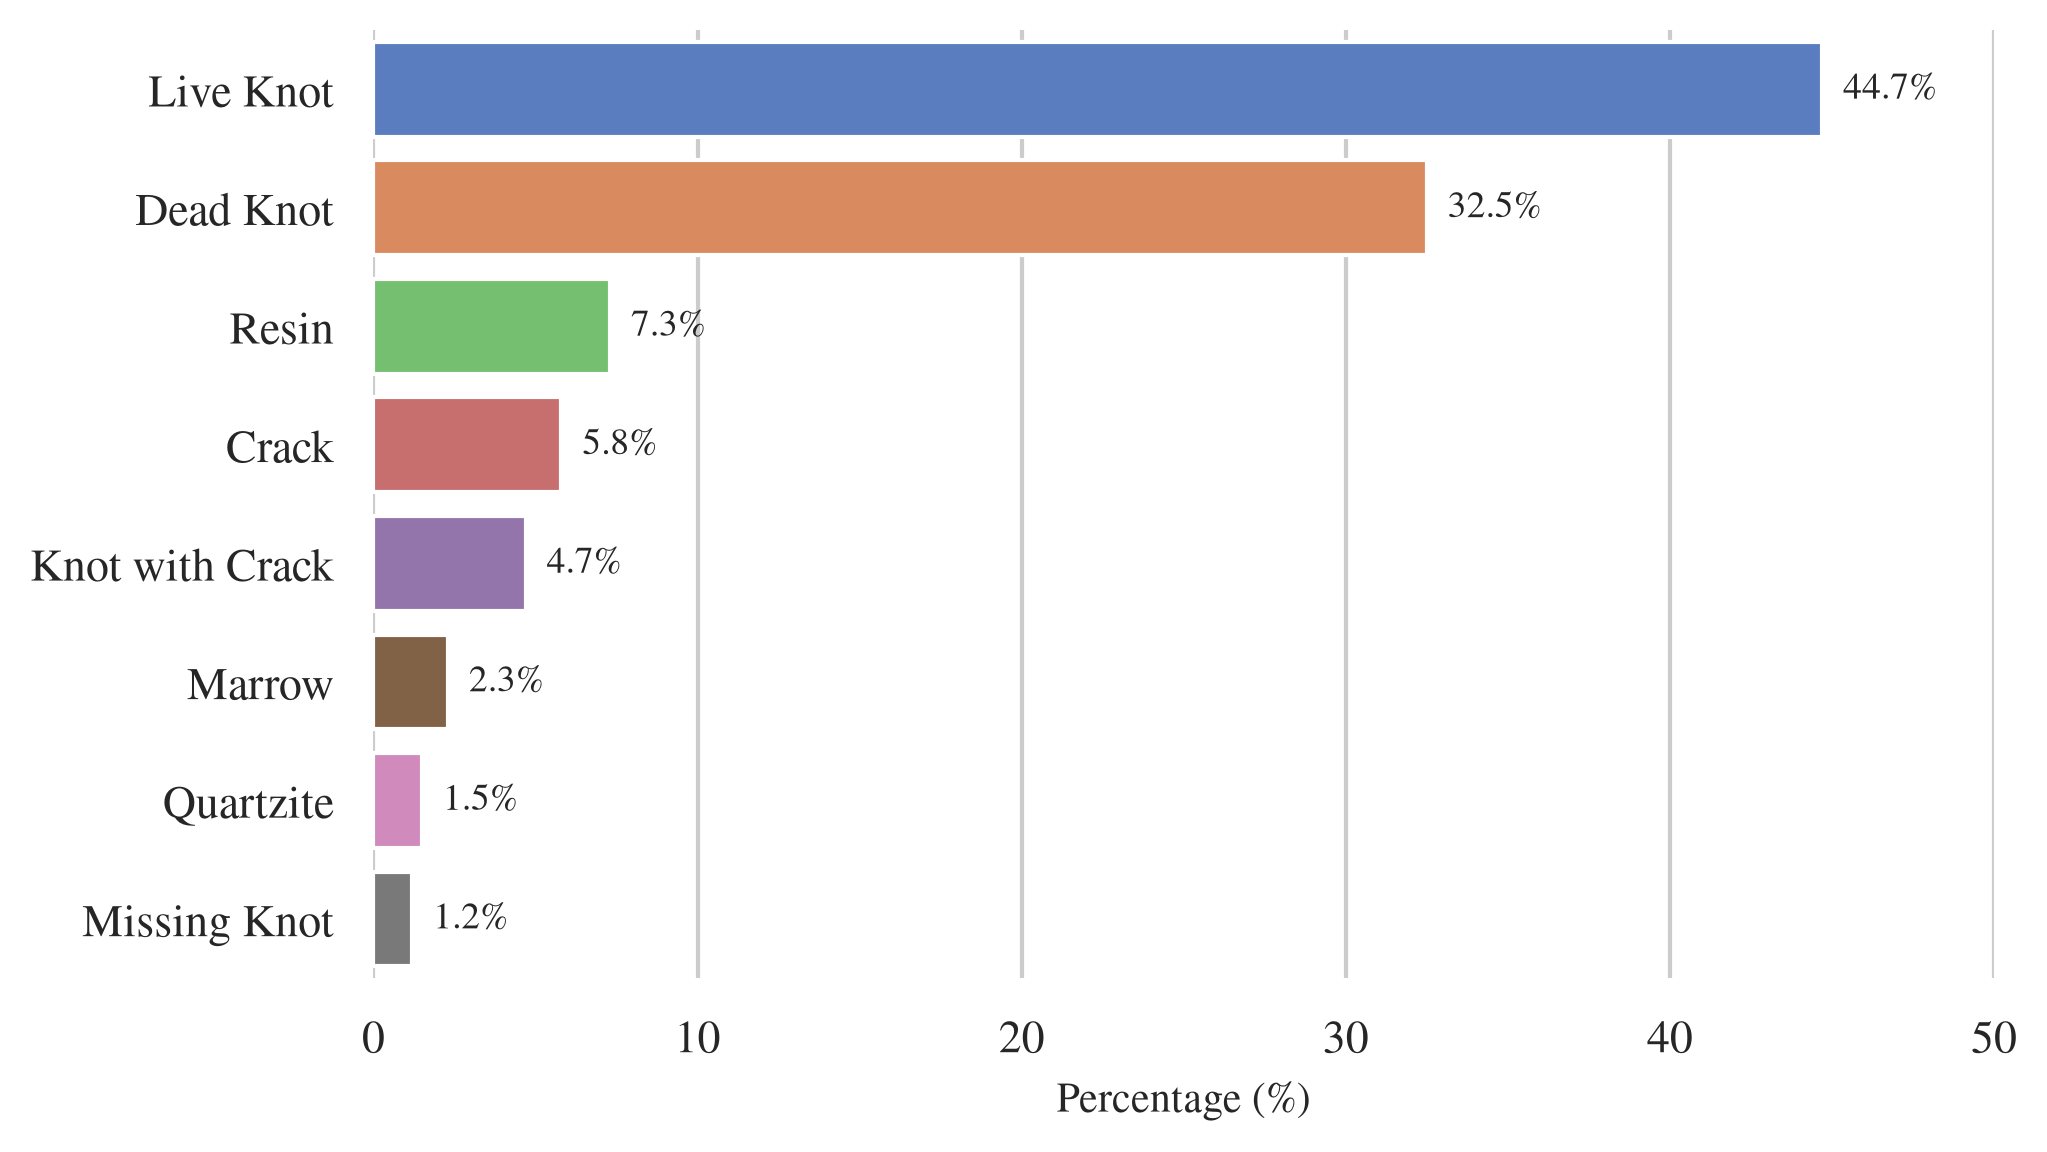
\includegraphics[width=\textwidth]{figures/dataset/barchart_classes.png}
\caption{Defect class distribution in the filtered dataset \cite{Nomihsa2024KaggleWood}: Live Knot, Dead Knot, Resin, Crack, Knot with Crack, Marrow, Quartzite, and Missing Knot.}
\label{fig:piechart-clases}
\end{figure*}

The annotations provide normalized bounding box coordinates in YOLO format. The class distribution reflects real industrial production conditions \cite{Kodytek2022Dataset}. Majority categories correspond to Live Knot with 3,949 annotations (44.4\%) and Dead Knot with 2,865 annotations (32.2\%), combining 76.6\% of the set. Intermediate categories include Resin with 642 annotations (7.2\%), Crack with 509 annotations (5.7\%), and Knot with Crack with 463 annotations (5.2\%). Minority categories comprise Marrow with 204 annotations (2.3\%), Quartzite with 144 annotations (1.6\%), and Missing Knot with 112 annotations (1.3\%). The calculated imbalance ratio reaches an approximate value of 35.3. Figure~\ref{fig:defectos-ejemplo} shows representative examples of each class.

\begin{figure*}[t]
\centering
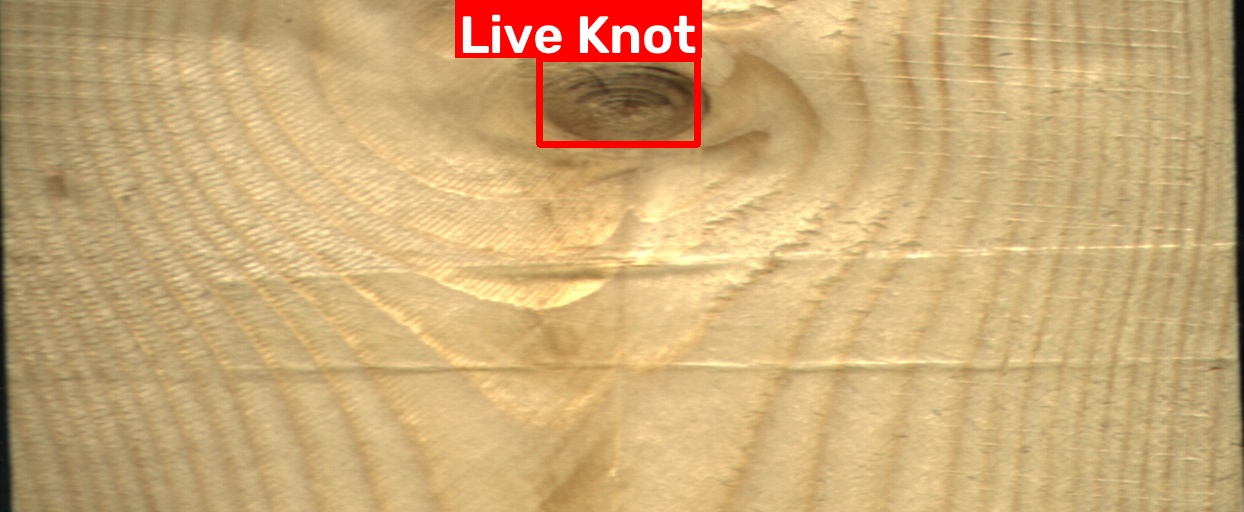
\includegraphics[width=0.24\textwidth]{figures/dataset/Live_Knot.jpg}\hfill
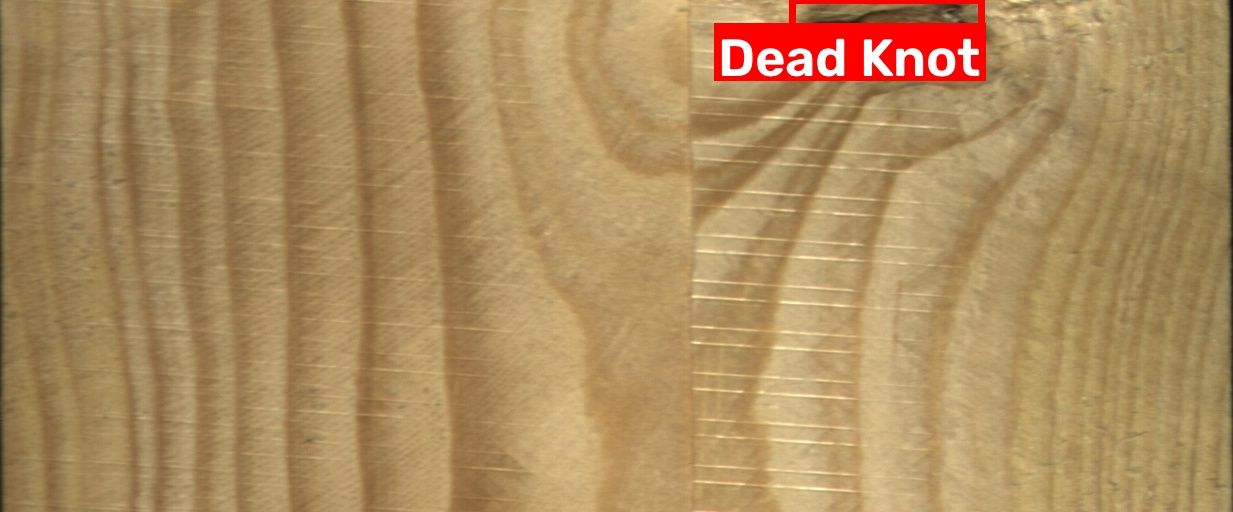
\includegraphics[width=0.24\textwidth]{figures/dataset/Dead_Knot.jpg}\hfill
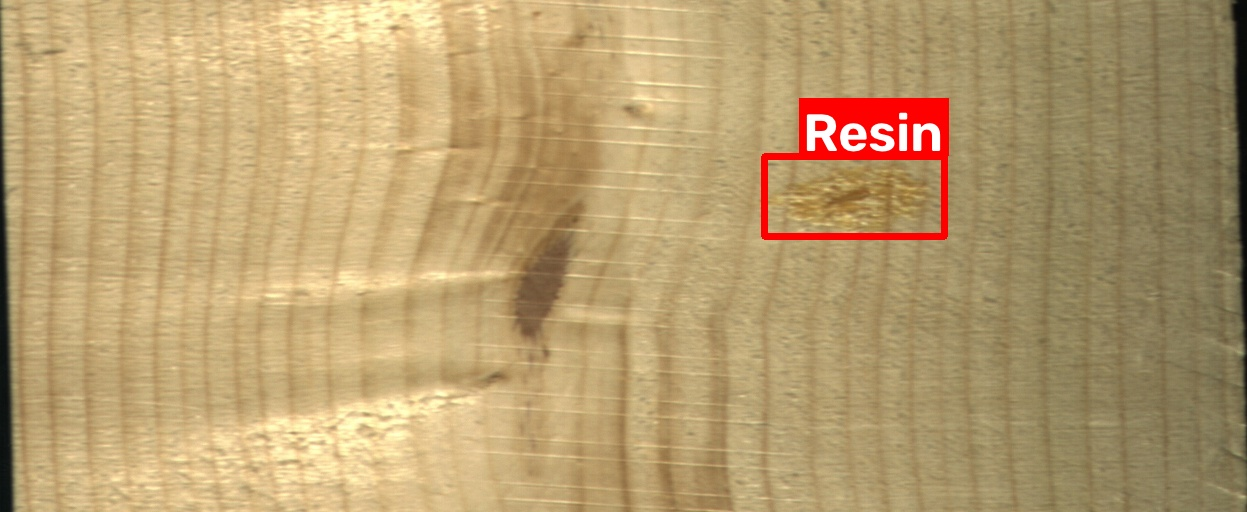
\includegraphics[width=0.24\textwidth]{figures/dataset/resin.jpg}\hfill
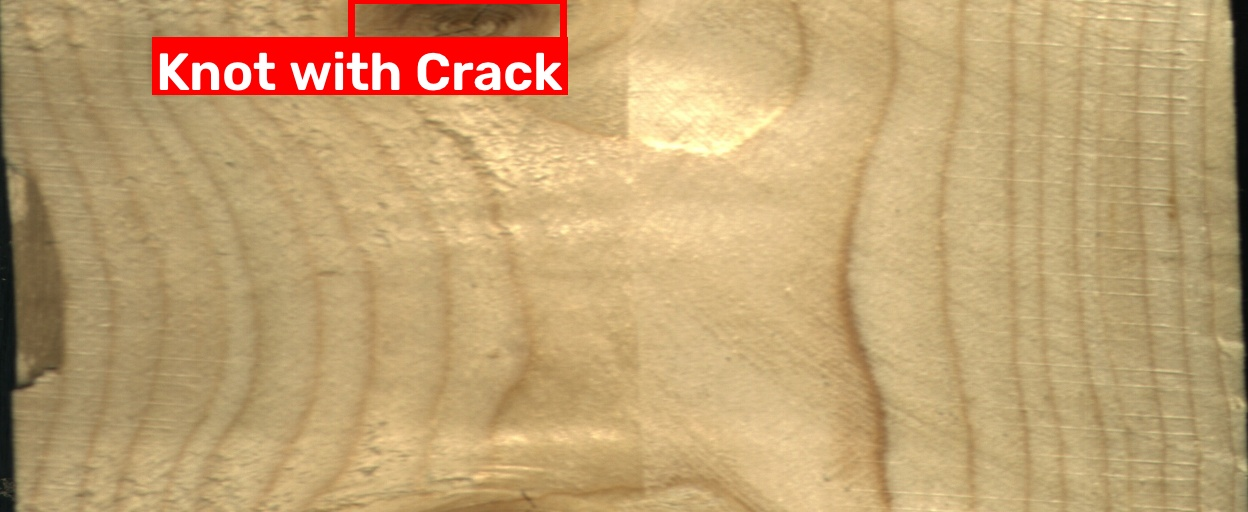
\includegraphics[width=0.24\textwidth]{figures/dataset/knot_with_crack.jpg}\\[4pt]
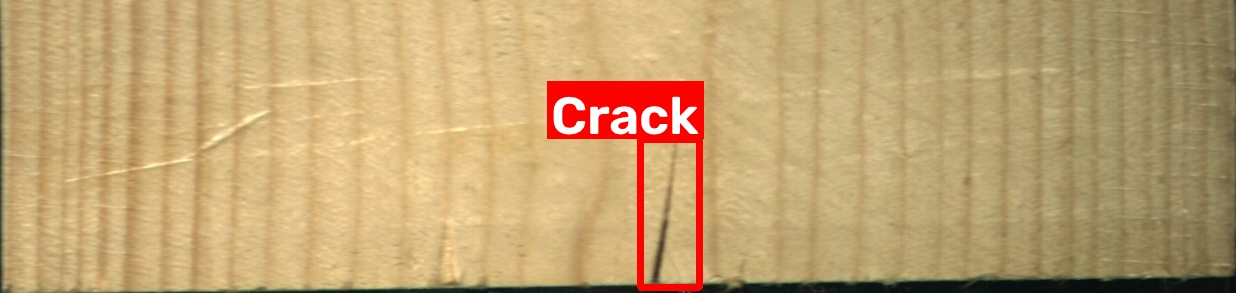
\includegraphics[width=0.24\textwidth]{figures/dataset/Crack.jpg}\hfill
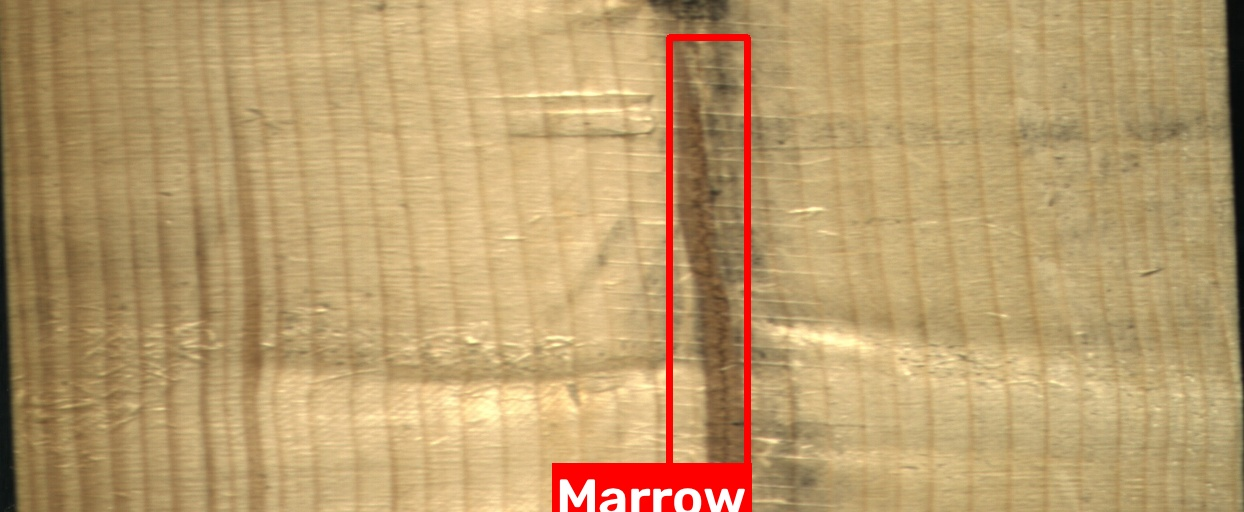
\includegraphics[width=0.24\textwidth]{figures/dataset/Marrow.jpg}\hfill
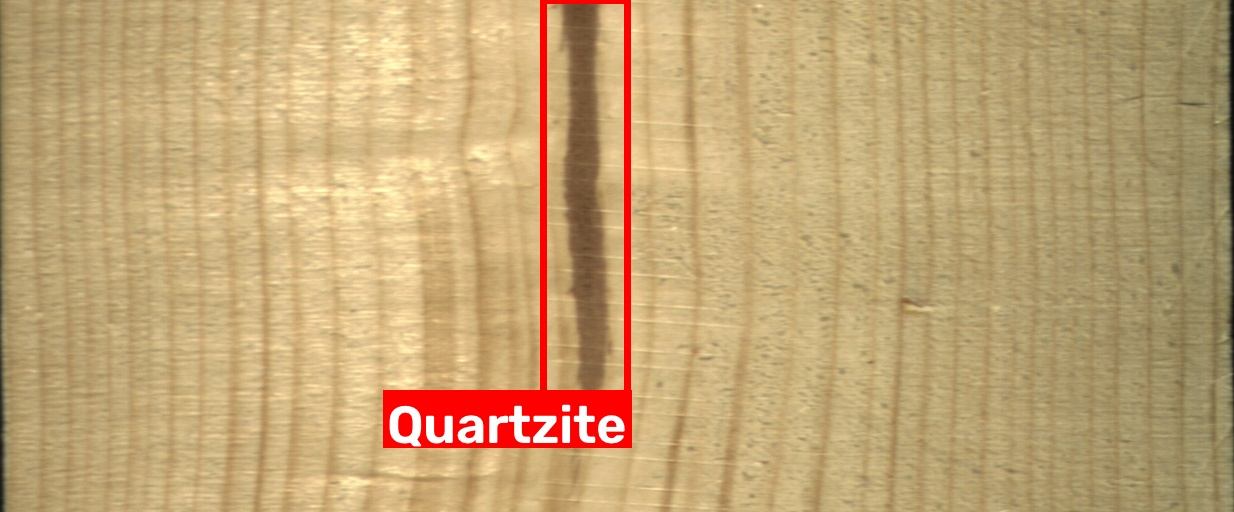
\includegraphics[width=0.24\textwidth]{figures/dataset/Quartzity.jpg}\hfill
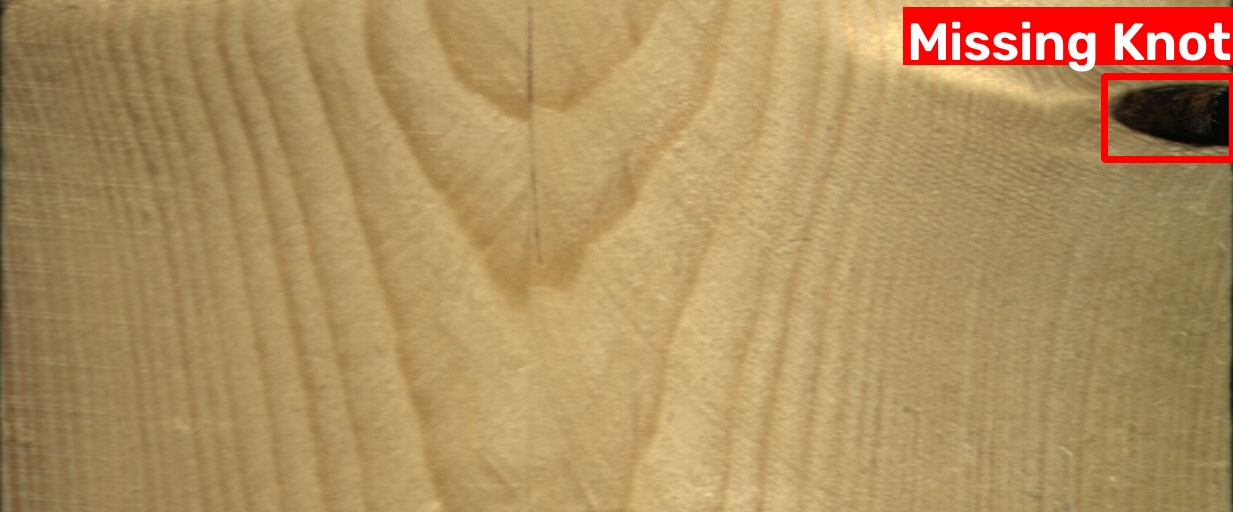
\includegraphics[width=0.24\textwidth]{figures/dataset/Knot_missing.jpg}
\caption{Examples of the eight defect classes annotated in the wood dataset \cite{Nomihsa2024KaggleWood}: Live Knot, Dead Knot, Resin, Knot with Crack, Crack, Marrow, Quartzite, and Missing Knot (left to right, top to bottom).}
\label{fig:defectos-ejemplo}
\end{figure*}

\subsection{Proposed Method}
\label{sec:proposed}

The proposed method implements a five-stage experiment pipeline designed to ensure reproducibility and fair comparability between configurations. The stages comprise: (1) data preparation, (2) data augmentation, (3) model training, (4) evaluation, and (5) results analysis. Figure~\ref{fig:pipeline} overviews the flow with the essential operation of each stage; the surrounding text details parameters and design choices. The entire pipeline configuration is managed through typed Pydantic models that guarantee parameter validation at compile time \cite{colvin2024pydantic}. The command-line interface allows customization of any nested parameter through dot notation, facilitating reproducible experimentation. All random number generators (Python, NumPy, PyTorch) are seeded from a single master seed with fixed per-stage stream ids, however, cudnn benchmarking and TF32 remain enabled.

\begin{figure*}[t]
\centering
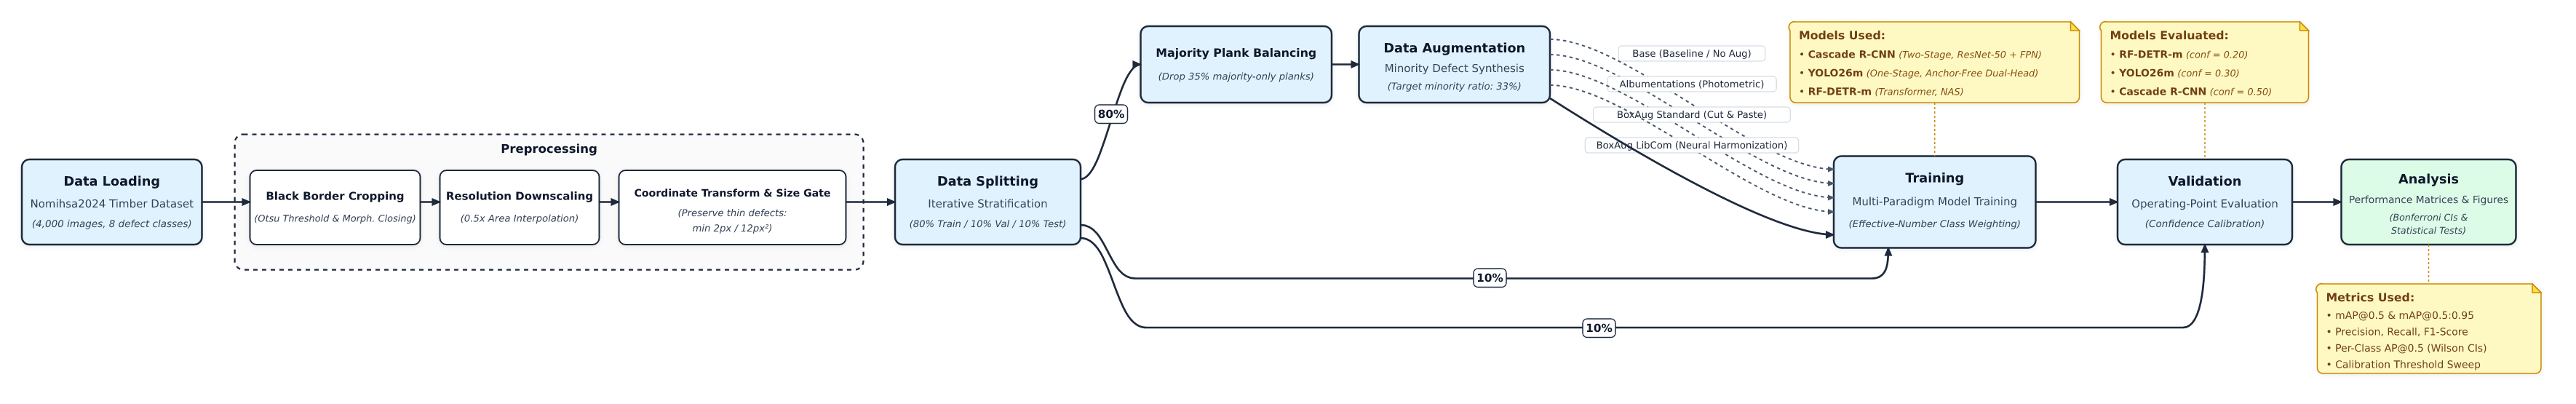
\includegraphics[width=\textwidth]{figures/methods/pipeline.png}
\caption{Overview of the proposed five-stage experimental pipeline for timber defect detection benchmarking.}
\label{fig:pipeline}
\end{figure*}

The data preparation stage applies three sequential operations on the raw dataset. First, black edges are cropped through Otsu thresholding segmentation \cite{otsu1979threshold} and morphological closing operations, isolating the valid region of the wood plank. Second, images are reduced to half their original resolution through area interpolation. Third, bounding box annotations are transformed to the resulting coordinate space and filtered by a three-rule size gate (minimum absolute dimension 2.0~px unless area reaches 12.0~px$^2$ or the major dimension reaches 6.0~px, preserving thin cracks while dropping unusable specks). The resulting set is partitioned into 80\% training, 10\% validation, and 10\% test through greedy iterative stratification that preserves class distribution in each partition \cite{kubat2000addressing}. To alleviate imbalance, 35\% of training planks containing only the two majority defect classes are then dropped; this intentionally shifts training priors away from the natural validation and test distributions, so reduced majority-class scores are expected even when the balancing works.

Three augmentation strategies were evaluated designed to mitigate class imbalance, aimed at achieving a 33\% ratio between the minority and majority class. Each strategy grows the training set by synthesizing minority-class instances, so augmented training sizes differ from the original by design and dataset size is reported per strategy. For the paradigm comparison, three representative architectures of each object detection approach were configured. Evaluation is performed on the test set of 400 images using COCO-standard mAP@0.5 and mAP@0.5:0.95, per-class AP@0.5, and operating-point precision, recall, and F1 at per-model calibrated confidence thresholds. Inference time is measured by averaging total processing time across all test set images.

Per-class uncertainty is quantified at the same operating points. For each class $c$, TP, FP, and FN counts come from the $\text{IoU}\ge 0.5$ greedy operating-point matching, and per-class precision and recall are treated as binomial proportions; simultaneous 95\% family-wise coverage over the $K = 8$ defect classes is obtained with the Bonferroni correction, reporting each class with a Wilson score interval at level $1 - 0.05/8 = 99.375\%$ ($z = 2.73$), i.e. $\mathrm{CI}_c = \mathrm{Wilson}(x_c, n_c; z_{1-0.05/16})$, with a dash shown when $n_c = 0$. Because matching is restricted to the same class, a cross-class mislabel surfaces as a false positive of the predicted class plus a false negative of the true class rather than as an off-diagonal confusion entry.

All architectures are trained with effective-number class weighting \cite{cui2019classbalanced} injected into each model's classification loss. While techniques such as Focal Loss \cite{lin2017focal} and Seesaw Loss \cite{wang2021seesaw} target the same imbalance, the study fixes a single loss-level treatment so that augmentation effects remain attributable, leaving alternative loss strategies as future work. Each model is evaluated at its own calibrated operating point while inferring at its own training resolution, so neither input-size handling nor a fixed confidence cutoff can favor any paradigm.

The augmentation stage applies three strategies targeting a 33\% minority-to-majority ratio (mode descriptions in Section~\ref{sec:fundamentals}). Albumentations with class balancing selectively augments images of rare classes with six transforms: horizontal flip (0.5), vertical flip (0.5), rotation-scale-translation (0.5), random contrast-brightness (0.4), color variation (0.3), and Gaussian blur (0.2). It is chosen as the photometric baseline because its transforms preserve labels while supporting bounding boxes \cite{buslaev2020albumentations}.

Standard BoxAug crops tail-class instances from an object bank, applies scale jitter (0.8--1.2), rotation, flipping, cropping, noise, and morphological operations, and pastes them at guide-validated positions (Missing Knot at edges, Quartzite central). Each run regenerates from a clean training copy with capped placement retries. It is chosen as the object-level oversampling arm because copy-paste is data-efficient for rare categories \cite{ghiasi2021simple} and a recommended imbalance remedy \cite{shorten2019augmentation}.

BoxAug with LibCom repeats the same procedure but replaces direct insertion with LibCom neural harmonization \cite{niu2021making}, restricted to scale jitter and flips without pixel noise. It is chosen to test whether harmonized composition with pixel-wise color equalization \cite{Guerreiro_2023_CVPR} removes the pasting discontinuities of the classic arm.

Cascade R-CNN (ResNet-50 + FPN \cite{cai2018cascade}) is trained for 12 epochs per the canonical MMDetection 1x schedule \cite{mmdetection}, with AdamW (lr 1e-4, wd 1e-4) adapted for single-GPU fine-tuning---the official 1x uses SGD with lr 0.02---batch size 8, $960\times 384$ keep-ratio input, LinearLR warmup plus MultiStepLR, COCO-bbox validation each epoch, patience 8 with min-delta 0.005, keeping the best-mAP checkpoint. The short schedule is justified by the cascaded heads (IoU 0.5/0.6/0.7) gaining about 4 AP points over the FPN baseline \cite{cai2018cascade}, and two-stage detectors are a proven but slower wood-defect option \cite{cwbyolo2024}.

YOLO26m (anchor-free, NMS-free dual-head \cite{jocher2026ultralyticsyolo26unifiedrealtime}) trains 50 epochs (patience 50, checkpoint every 5) at $960\times 384$, batch size 16, lr0 0.01, AMP FP16. The lr0 value is the Ultralytics default and 50 epochs is a reduced COCO-pretrained fine-tuning budget (default 100). The regime mirrors CWB-YOLOv8 on wood (lr0 0.01, patience 50, mAP@0.5 of 0.892 without overfitting \cite{cwbyolo2024}) and the YOLOv5m COCO-pretrain plus fine-tune protocol that reached 97.7\% F-score on sawn-timber knots \cite{fang2021yolov5knots}; the budget is ample against the 500--600 epochs needed from scratch \cite{jocher2026ultralyticsyolo26unifiedrealtime}.

RF-DETR-m \cite{robinson2026rfdetrneuralarchitecturesearch} trains on a $960\times 384$ canvas with batch size 8, AdamW with lr 1e-4 and wd 1e-4 (both official defaults), gradient checkpointing, up to 50 epochs with patience 15 and min-delta 0.005 per the official early-stopping example (actual 21--23 epochs, best validation epochs 6--11). The 5-epoch warmup is an explicit fine-tuning stabilizer (official default 0). The learning-rate choice matches the RF-DETR training hyperparameters that reach 48.0 COCO AP at nano scale \cite{robinson2026rfdetrneuralarchitecturesearch}; as a 2026 architecture, this study is its first reported use on wood.

The differing epoch budgets are intentional: MMDetection 1x (12 epochs) for Cascade R-CNN \cite{mmdetection}, a 50-epoch fine-tuning budget for YOLO26 against Ultralytics defaults, and up to 50 epochs with early stopping for RF-DETR per official guidance \cite{robinson2026rfdetrneuralarchitecturesearch}. Wall-clock budgets are comparable across paradigms (0.38 to 0.80 hours per configuration, see Figure~\ref{fig:tiempo-entrenamiento}) because per-epoch cost differs, so epoch counts cannot be compared directly. All three paradigms share the $960\times 384$ canvas, COCO-pretrained initialization, effective-number class weighting \cite{cui2019classbalanced}, and per-model calibrated operating points.

\begin{table*}[t]
\caption{Training hyperparameters per paradigm. Each parameter is reported with its value; provenance and deviations from framework defaults are justified in the text.}
\label{tab:tabla-hiperparametros}
\centering
\begin{tabular*}{\textwidth}{@{\extracolsep{\fill}}lll@{}}
\toprule
Model & Parameter & Value \\
\midrule
Cascade R-CNN (ResNet-50 + FPN) & Input resolution & $960\times 384$, keep-ratio \\
& Batch size & 8 \\
& Optimizer & AdamW (adapted for single-GPU fine-tuning; official 1x uses SGD) \\
& Learning rate & 1e-4 \\
& Weight decay & 1e-4 \\
& Schedule & LinearLR warmup + MultiStepLR \\
& Epoch budget & 12 (MMDetection 1x), patience 8, min-delta 0.005 \\
\addlinespace
YOLO26m (anchor-free, dual-head) & Input resolution & $960\times 384$ rectangular \\
& Batch size & 16 \\
& Optimizer & Ultralytics default (auto), MuSGD design \\
& Initial learning rate (lr0) & 0.01 (Ultralytics default) \\
& Precision & AMP FP16 \\
& Epoch budget & 50, patience 50 (effectively off), checkpoint every 5 \\
\addlinespace
RF-DETR-m (NAS transformer) & Input canvas & $960\times 384$ rectangular \\
& Batch size & 8 \\
& Optimizer & AdamW (official default) \\
& Learning rate & 1e-4 (official default) \\
& Weight decay & 1e-4 (official default) \\
& Warmup & 5 epochs (explicit stabilization; official default 0) \\
& Memory & Gradient checkpointing \\
& Epoch budget & max 50, actual 21--23, patience 15, min-delta 0.005 \\
\bottomrule
\end{tabular*}
\end{table*}

Confidence thresholds are calibrated per model rather than fixed globally. A validation-split inference pass at 0.05 followed by a max-F1 sweep sets the operating point: 0.20 for RF-DETR (F1 0.695) and 0.30 for YOLO26 (F1 0.748), while Cascade R-CNN stays at 0.50. Test inference and metrics for all RF-DETR and YOLO26 configurations run at these thresholds. Calibration is required because rectangular training deflates RF-DETR output scores while preserving ranking quality: the same checkpoints score far lower at a fixed 0.50 cutoff through lost recall, not worse localization. Precision, recall, and F1 are therefore reported at each model's own operating point, while the mAP columns remain the ranking-based comparison.

%% ============================================================
%% 4. RESULTS
%% ============================================================

\section{Results}
\label{sec:results}

Figure~\ref{fig:matrix-map50} presents the mAP@0.5 performance matrix for the 12 model-augmentation strategy combinations. RF-DETR leads all four arms with values between 0.676 and 0.717, followed by Cascade R-CNN between 0.644 and 0.677, while YOLO26 is the tightest group between 0.592 and 0.618 with its unaugmented baseline on top. The strict-metric view in Figure~\ref{fig:matrix-map5095} preserves the order. Augmentation sensitivity is paradigm-specific rather than uniform: it helps Cascade, is mixed for RF-DETR, and is neutral to negative for YOLO26.

\begin{figure*}[t]
\centering
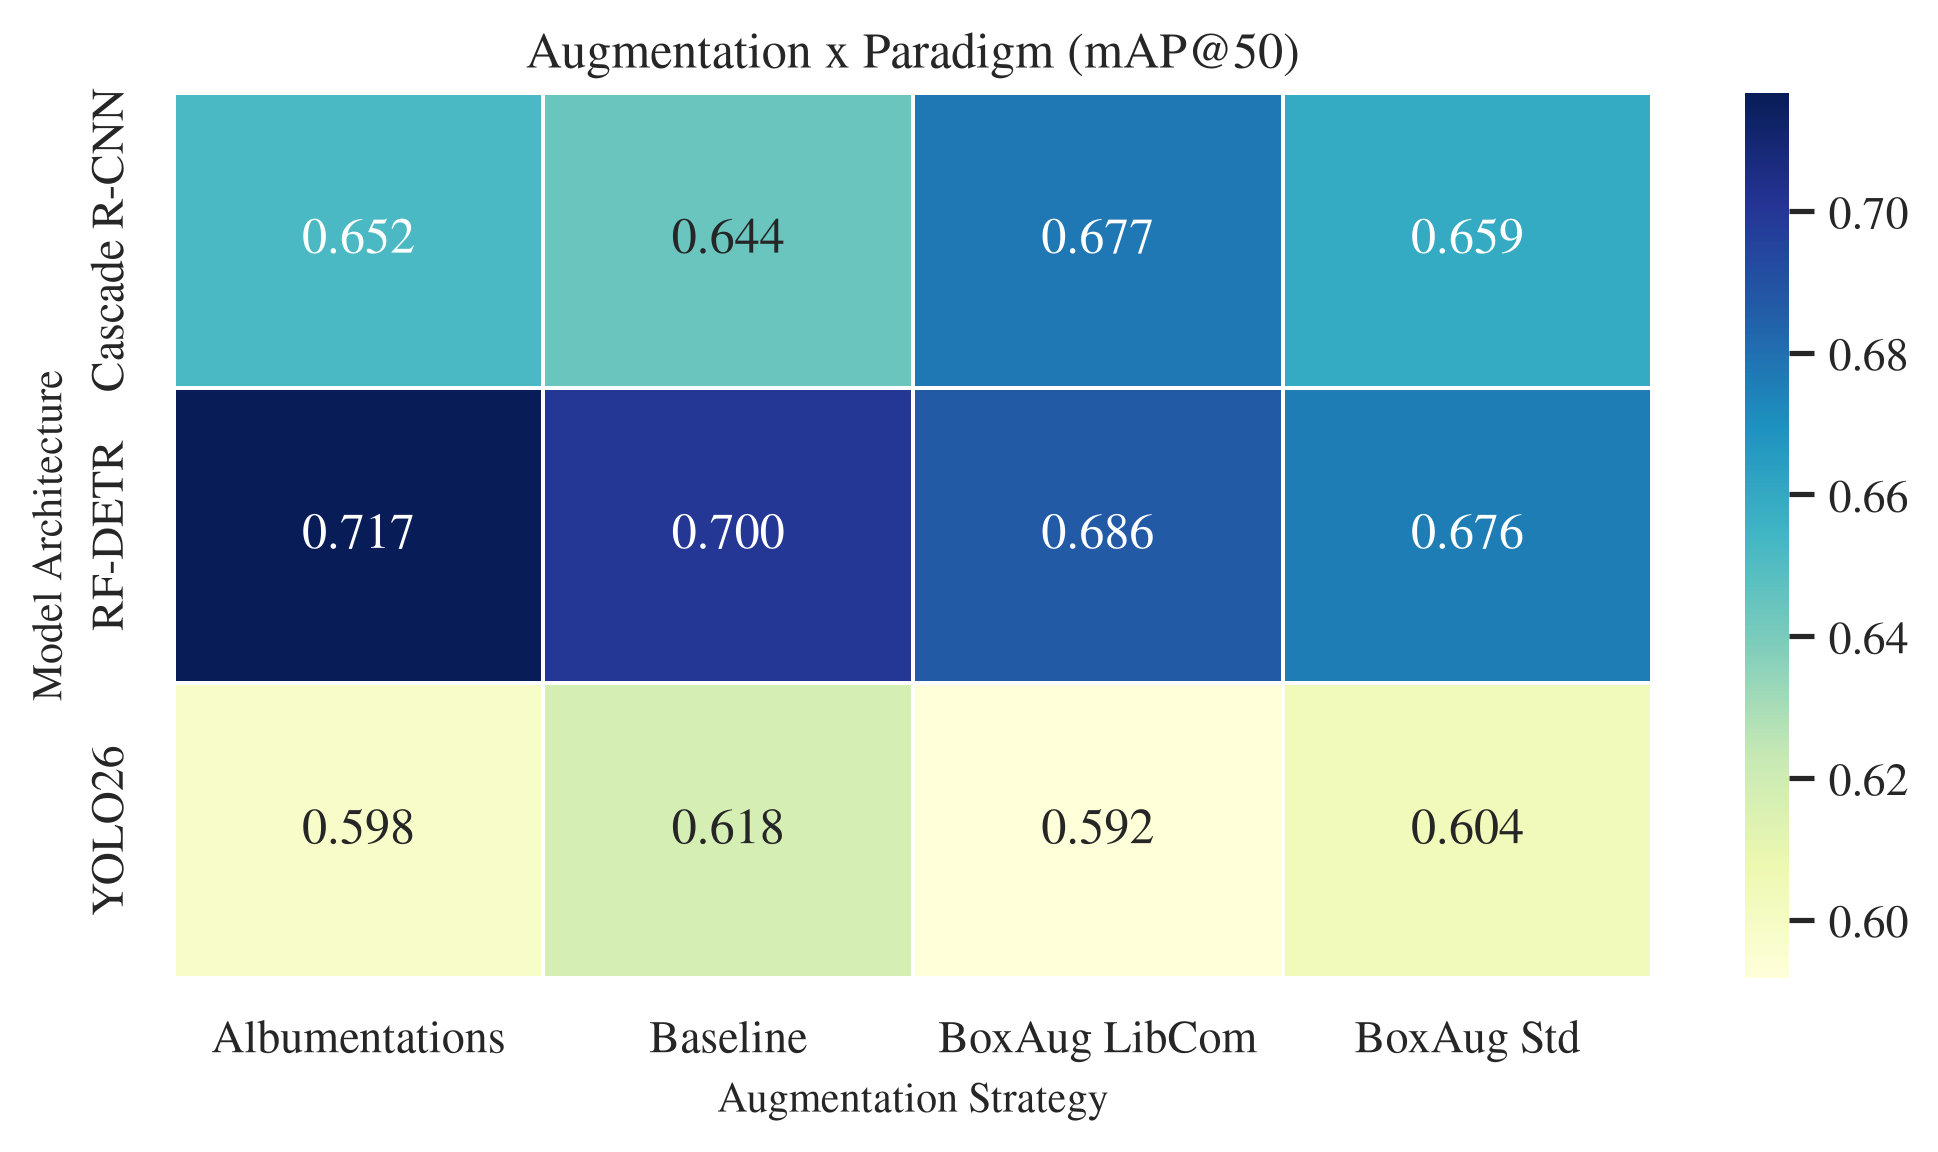
\includegraphics[width=\textwidth]{figures/results/aug_paradigm_map50_heatmap.png}
\caption{mAP@0.5 performance matrix intersecting three detection paradigms with four augmentation strategies.}
\label{fig:matrix-map50}
\end{figure*}

\begin{figure*}[t]
\centering
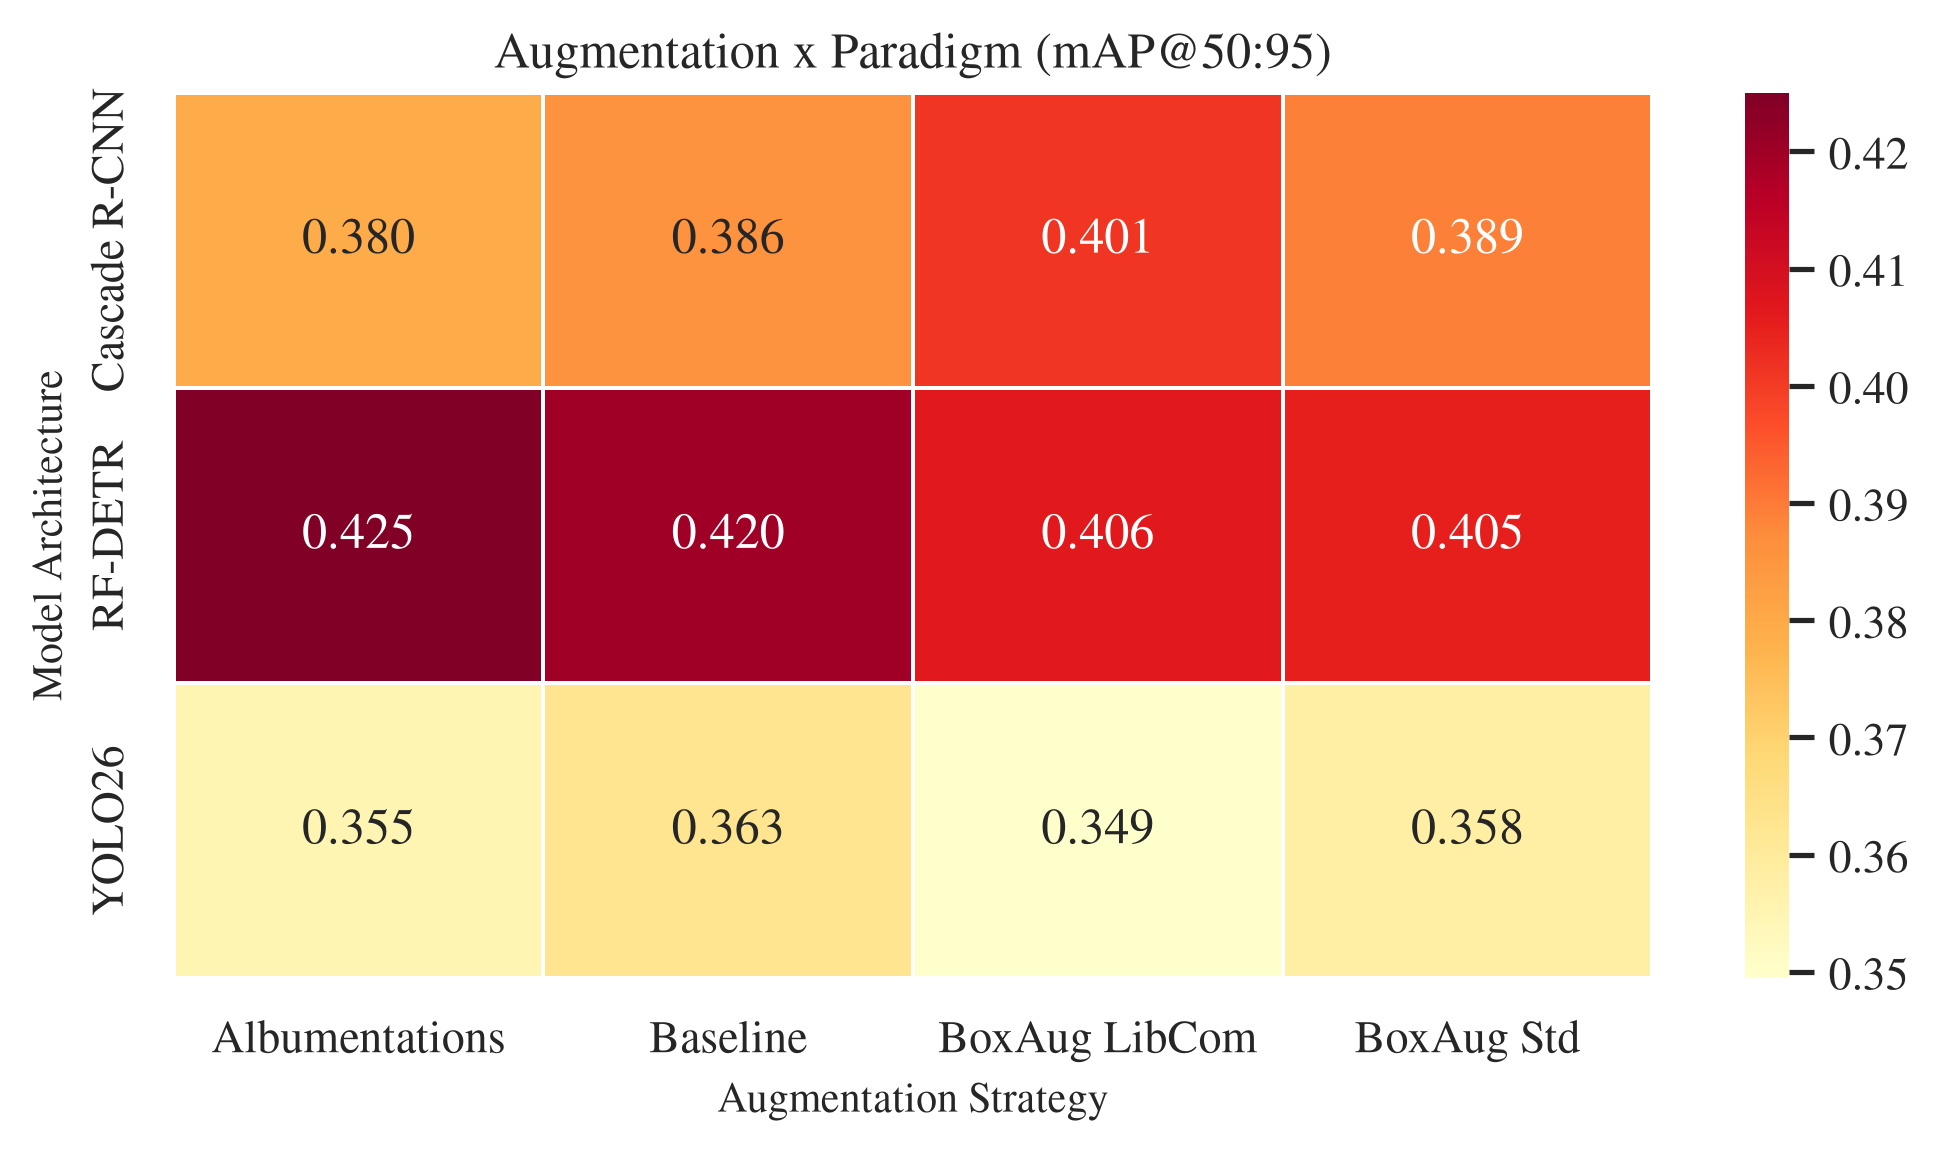
\includegraphics[width=\textwidth]{figures/results/aug_paradigm_map50_95_heatmap.png}
\caption{mAP@0.5:0.95 performance matrix for the same 12 configurations.}
\label{fig:matrix-map5095}
\end{figure*}

Table~\ref{tab:tabla-principal} summarizes the complete metrics for all 12 configurations. RF-DETR with Albumentations achieves the highest mAP@0.5 of 0.717 and the best mAP@0.5:0.95 of 0.425, while Cascade R-CNN with BoxAug LibCom reaches the highest precision of 0.811 and the best F1 of 0.798. YOLO26 baseline is the strongest of its family at mAP@0.5 of 0.618, with all three augmentation strategies scoring 0.592 to 0.604. These results place the transformer paradigm first on ranking metrics and the two-stage paradigm first on operating-point precision, while the one-stage paradigm shows no augmentation-driven gains under this protocol.

\begin{table*}[t]
\caption{Performance metrics on the test set for all 12 benchmark configurations.}
\label{tab:tabla-principal}
\centering
\begin{tabular*}{\textwidth}{@{\extracolsep{\fill}}llccccc@{}}
\toprule
Model & Augmentation & mAP@50 & mAP@50:95 & Precision & Recall & F1 \\
\midrule
Cascade R-CNN & Albumentations & 0.652 & 0.380 & 0.789 & 0.785 & 0.787 \\
Cascade R-CNN & Baseline       & 0.644 & 0.386 & 0.797 & 0.765 & 0.780 \\
Cascade R-CNN & BoxAug LibCom  & 0.677 & 0.401 & 0.811 & 0.785 & 0.798 \\
Cascade R-CNN & BoxAug Std     & 0.659 & 0.389 & 0.796 & 0.773 & 0.784 \\
\addlinespace
RF-DETR       & Albumentations & 0.717 & 0.425 & 0.684 & 0.782 & 0.730 \\
RF-DETR       & Baseline       & 0.700 & 0.420 & 0.667 & 0.794 & 0.725 \\
RF-DETR       & BoxAug LibCom  & 0.686 & 0.406 & 0.665 & 0.796 & 0.725 \\
RF-DETR       & BoxAug Std     & 0.676 & 0.405 & 0.660 & 0.794 & 0.721 \\
\addlinespace
YOLO26        & Albumentations & 0.598 & 0.355 & 0.742 & 0.748 & 0.745 \\
YOLO26        & Baseline       & 0.618 & 0.363 & 0.769 & 0.738 & 0.753 \\
YOLO26        & BoxAug LibCom  & 0.592 & 0.349 & 0.760 & 0.740 & 0.750 \\
YOLO26        & BoxAug Std     & 0.604 & 0.358 & 0.754 & 0.765 & 0.759 \\
\bottomrule
\end{tabular*}
\end{table*}

Figure~\ref{fig:delta-baseline} shows the impact of each augmentation strategy relative to the baseline for each model. Cascade R-CNN benefits from every strategy: Albumentations contributes +0.008, standard BoxAug +0.015, and BoxAug LibCom +0.033 absolute improvement in mAP@0.5. RF-DETR shows mixed behavior: Albumentations contributes +0.017, but standard BoxAug degrades performance by -0.024 and BoxAug LibCom by -0.013. YOLO26 shows no gain: Albumentations scores -0.019, BoxAug LibCom -0.026, and standard BoxAug -0.014, with the unaugmented baseline remaining its best configuration.

\begin{figure*}[t]
\centering
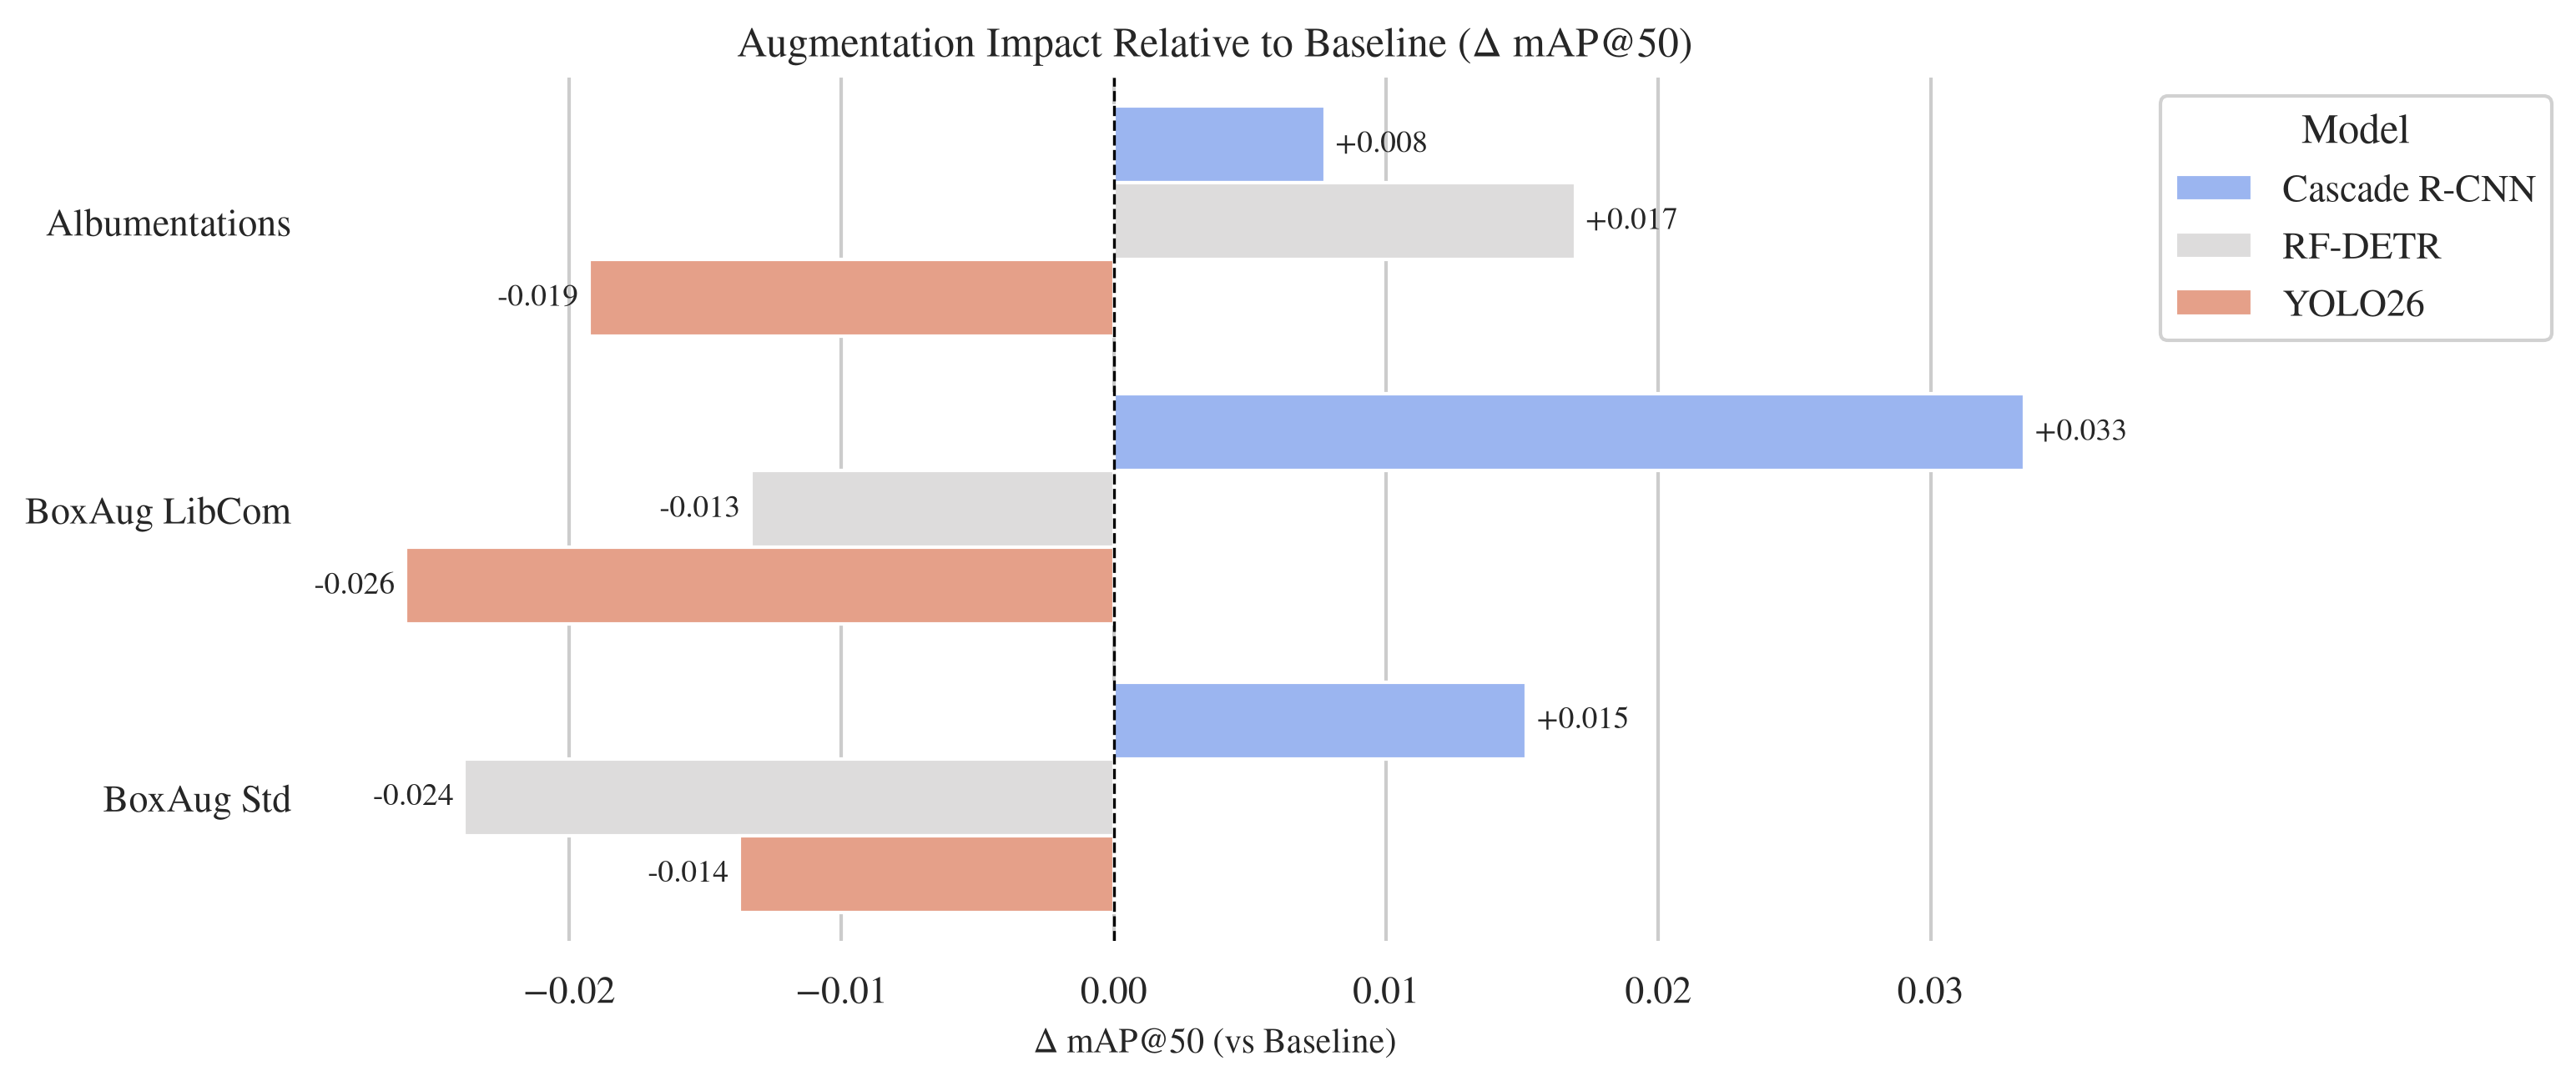
\includegraphics[width=\textwidth]{figures/results/aug_delta_vs_baseline.png}
\caption{Impact of augmentation strategies relative to baseline ($\Delta$ mAP@0.5).}
\label{fig:delta-baseline}
\end{figure*}

Figure~\ref{fig:heatmap-clase} presents the average AP per class at AP@0.5 for all 12 configurations. The easiest class is Marrow, with AP up to 0.910 with RF-DETR, while Quartzite is the hardest, with AP between 0.082 and 0.550. No configuration fails completely on any class. Live Knot and Dead Knot show AP values of 0.651 to 0.781 despite being the majority classes, suggesting high intra-class variance.

\begin{figure*}[t]
\centering
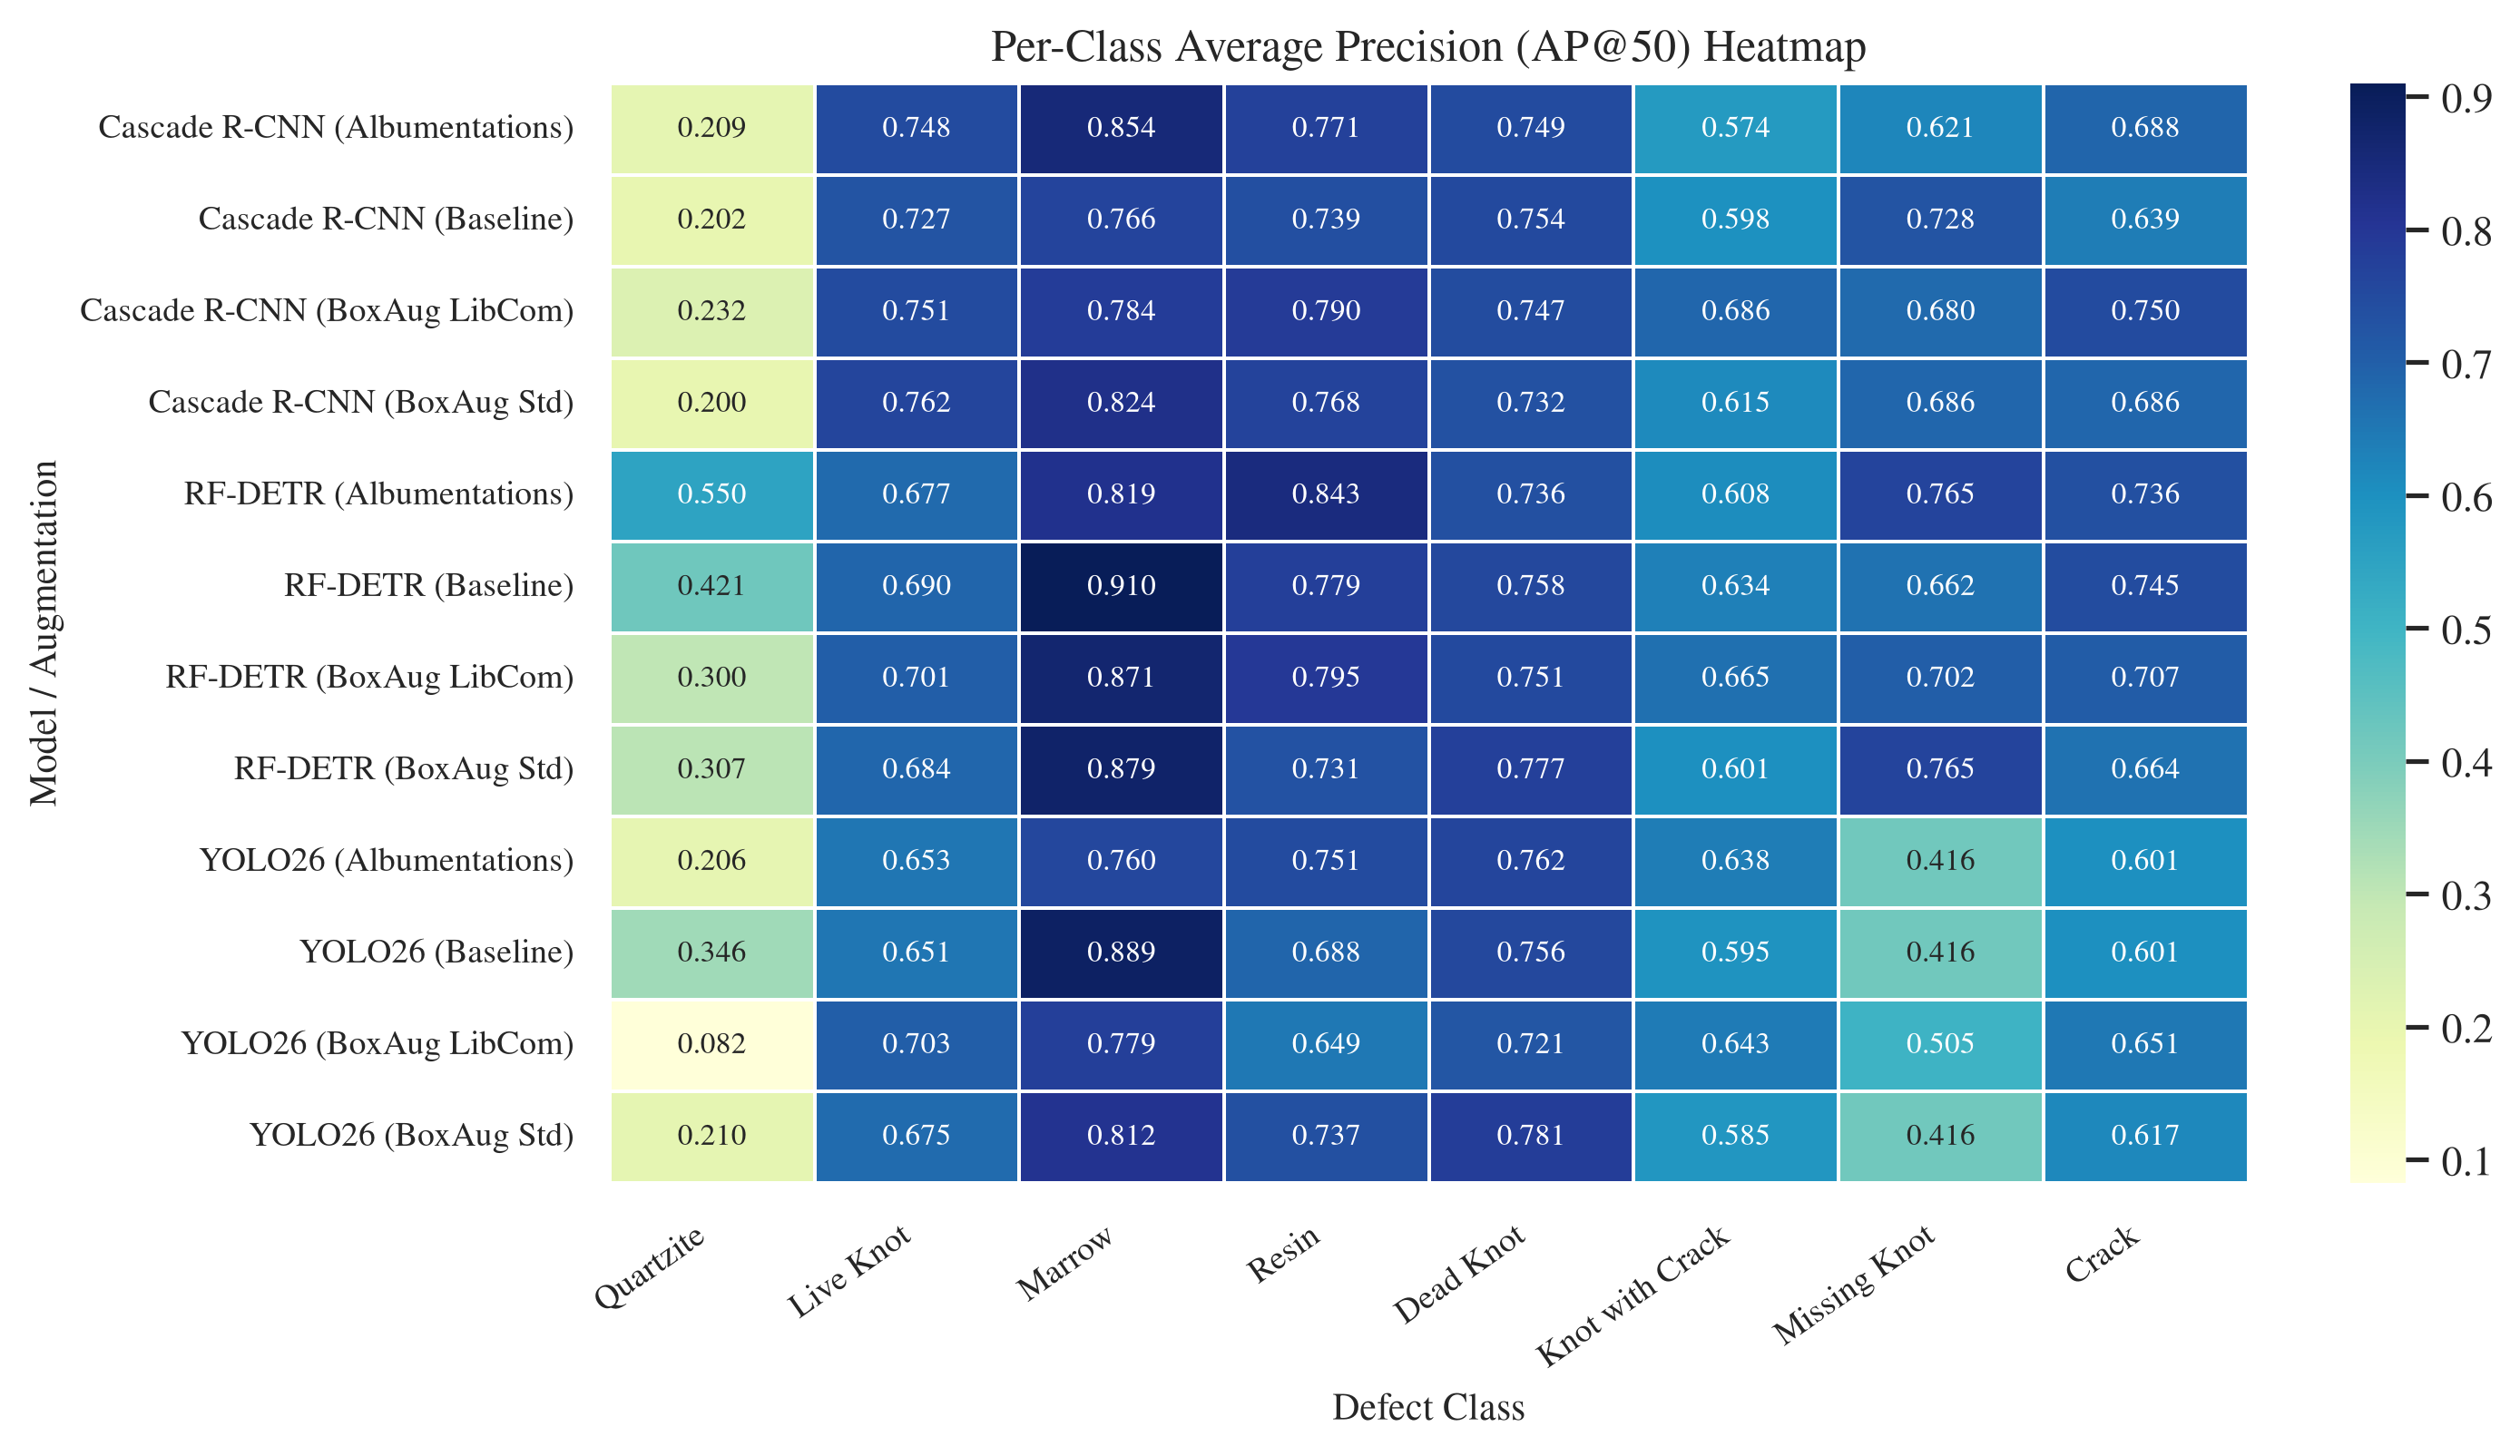
\includegraphics[width=\textwidth]{figures/results/per_class_ap_heatmap.png}
\caption{Heatmap of average precision per defect class (AP@0.5).}
\label{fig:heatmap-clase}
\end{figure*}

Figure~\ref{fig:heatmap-clase-5095} presents the same per-class breakdown under the AP@0.5:0.95 metric. The class ordering is preserved: Marrow remains the easiest class at 0.499 to 0.639 and Quartzite the hardest at 0.064 to 0.285. The metric compresses the score range, most visibly on the majority classes, as Live Knot and Dead Knot drop from 0.651 to 0.781 at AP@0.5 to 0.297 to 0.449, indicating that these high-variance defects are detected but poorly localized. The weakest cell is YOLO26 with BoxAug LibCom on quartzite at 0.064, against 0.255 for its unaugmented baseline, showing that pasted augmentation degrades rare-class localization for the one-stage paradigm. RF-DETR leads six of eight classes under the metric, with its best cells on marrow at 0.639 (BoxAug Std) and Knot\_missing at 0.502 (Albumentations).

\begin{figure*}[t]
\centering
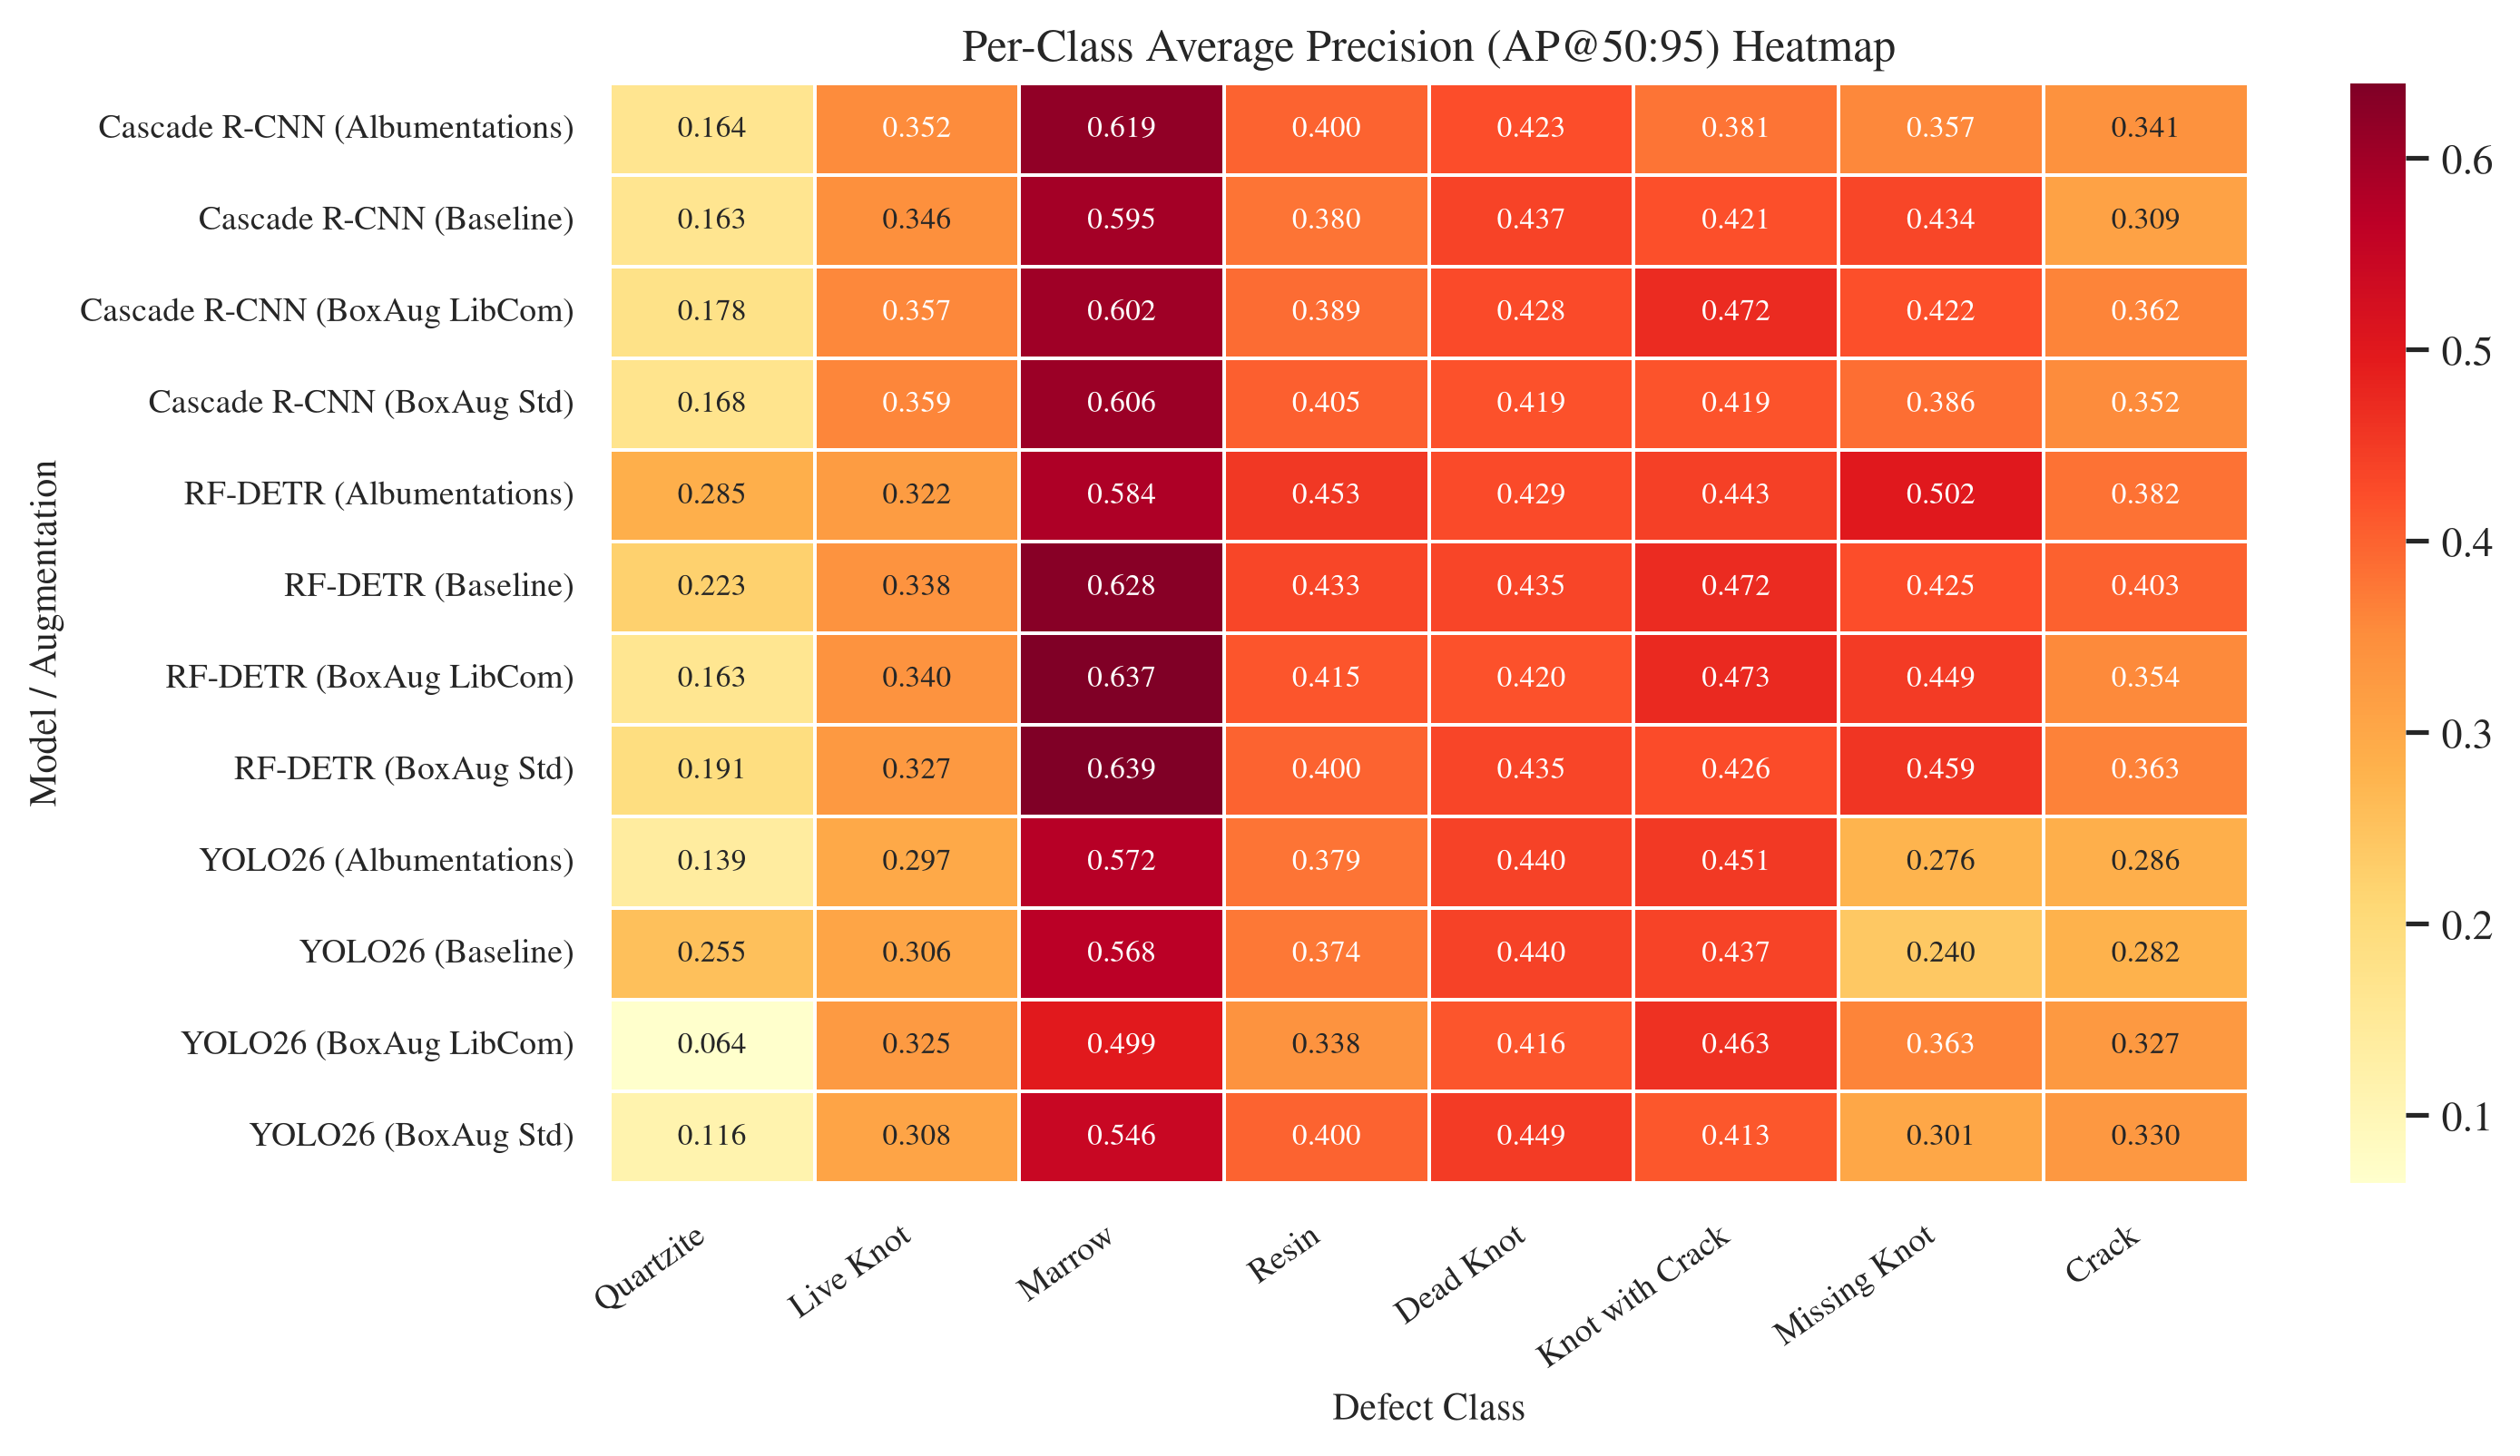
\includegraphics[width=\textwidth]{figures/results/per_class_ap50_95_heatmap.png}
\caption{Heatmap of average precision per defect class (AP@0.5:0.95).}
\label{fig:heatmap-clase-5095}
\end{figure*}

Table~\ref{tab:tabla-bonferroni} and Figure~\ref{fig:recall-bonferroni} report per-class recall with simultaneous 95\% CIs for the best configuration of each paradigm. Abundant classes give narrow intervals (Live Knot, $n = 395$: recall 0.729--0.792 with widths 0.111--0.122), while rare classes span tens of points (Quartzite, $n = 15$: 0.400--0.733 with widths 0.533--0.576; Missing Knot, $n = 12$: widths up to 0.614), so rank orders among rare classes are not statistically distinguishable: the Quartzite gap between RF-DETR (0.733) and YOLO26 (0.400) overlaps across all three intervals. Precision shows the same pattern, with Cascade R-CNN keeping the narrowest majority-class intervals (Live Knot 0.853 [0.795, 0.896], Dead Knot 0.905 [0.841, 0.945]) while rare-class intervals overlap.

\begin{table*}[t]
\caption{Per-class recall with simultaneous 95\% family-wise CIs (Bonferroni) for the best configuration of each paradigm, with test support $n$.}
\label{tab:tabla-bonferroni}
\centering
\begin{tabular*}{\textwidth}{@{\extracolsep{\fill}}lcccc@{}}
\toprule
Class & RF-DETR (Alb.) & Cascade (LibCom) & YOLO26 (Base.) & $n$ \\
\midrule
Quartzite & 0.733 [0.389, 0.922] & 0.467 [0.190, 0.766] & 0.400 [0.149, 0.718] & 15 \\
Live Knot & 0.754 [0.691, 0.809] & 0.792 [0.731, 0.843] & 0.729 [0.664, 0.786] & 395 \\
Marrow & 0.857 [0.561, 0.966] & 0.857 [0.561, 0.966] & 0.905 [0.614, 0.983] & 21 \\
Resin & 0.891 [0.741, 0.959] & 0.813 [0.649, 0.910] & 0.703 [0.533, 0.831] & 64 \\
Dead Knot & 0.767 [0.692, 0.828] & 0.763 [0.688, 0.825] & 0.788 [0.715, 0.846] & 287 \\
Knot with Crack & 0.787 [0.591, 0.905] & 0.766 [0.568, 0.891] & 0.702 [0.503, 0.846] & 47 \\
Missing Knot & 0.833 [0.441, 0.969] & 0.750 [0.369, 0.939] & 0.417 [0.142, 0.756] & 12 \\
Crack & 0.922 [0.758, 0.978] & 0.902 [0.733, 0.969] & 0.706 [0.515, 0.845] & 51 \\
\bottomrule
\end{tabular*}
\end{table*}

\begin{figure*}[t]
\centering
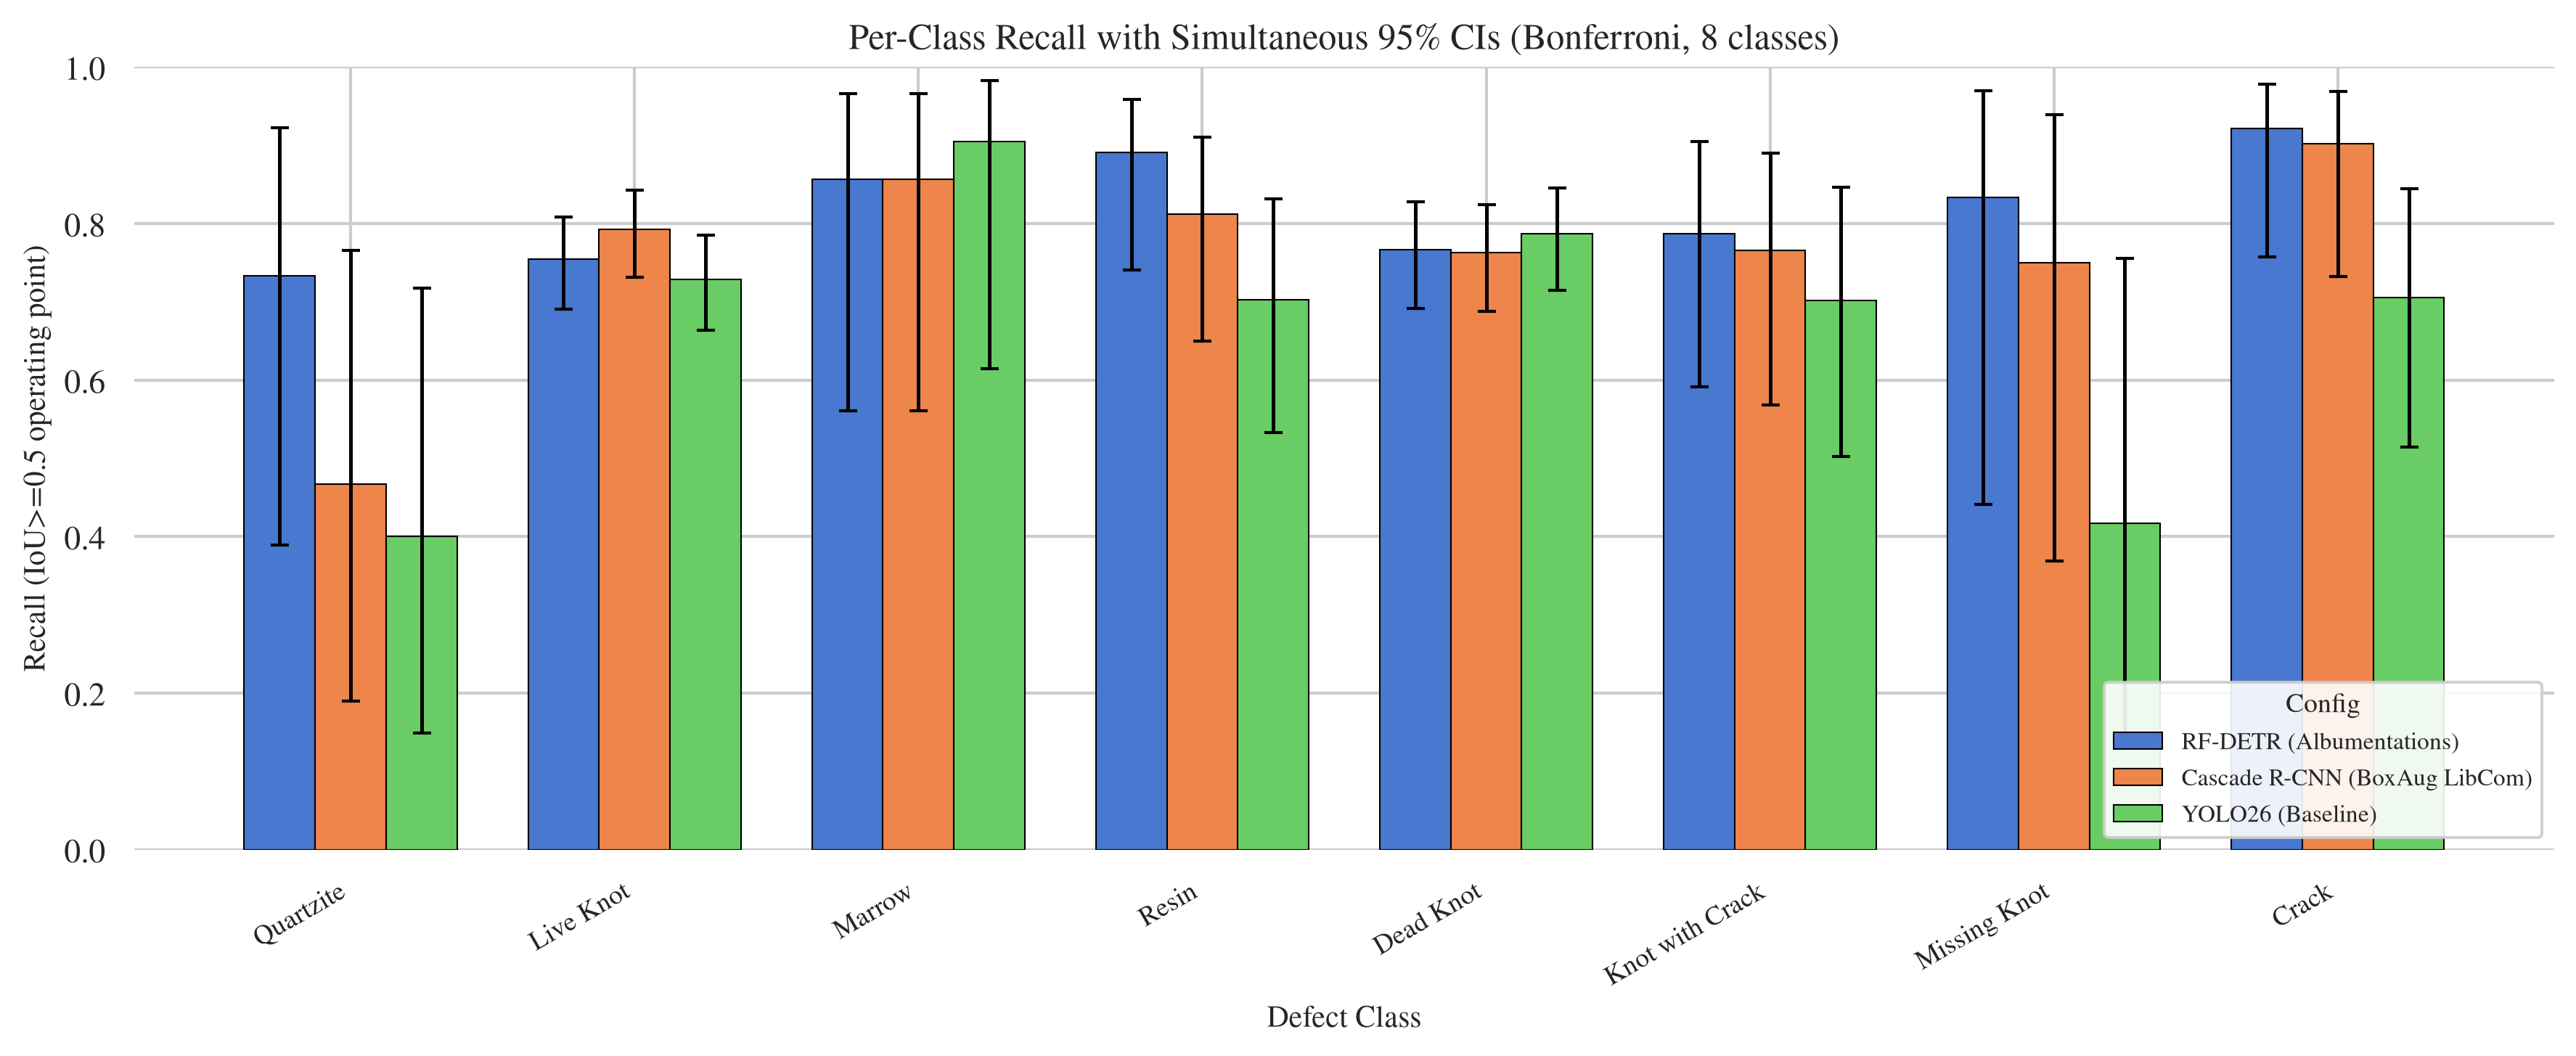
\includegraphics[width=\textwidth]{figures/results/per_class_recall_bonferroni.png}
\caption{Per-class recall with Bonferroni-corrected simultaneous 95\% family-wise confidence intervals for the best configuration of each paradigm.}
\label{fig:recall-bonferroni}
\end{figure*}

Figure~\ref{fig:inference-panel} shows ground-truth-annotated representative instances (red boxes) for the eight defect classes together with the best AP@0.5 across the 12 configurations. The panel visualizes the difficulty spectrum behind the numbers: the distinctive central-line pattern of Marrow (0.91) contrasts with the low contrast of Quartzite against wood grain (0.55, hardest class), while Missing Knot instances cluster at plank edges where operating-point recall intervals are widest ($n = 12$, widths up to 0.614). Characteristic failure modes follow from the operating-point counts: quartzite false positives arise from grain confusion (RF-DETR quartzite precision spans 0.133--0.501), and cross-class knot confusions surface as paired false positives and false negatives rather than off-diagonal entries (see Section~\ref{sec:proposed}).

\begin{figure*}[t]
\centering
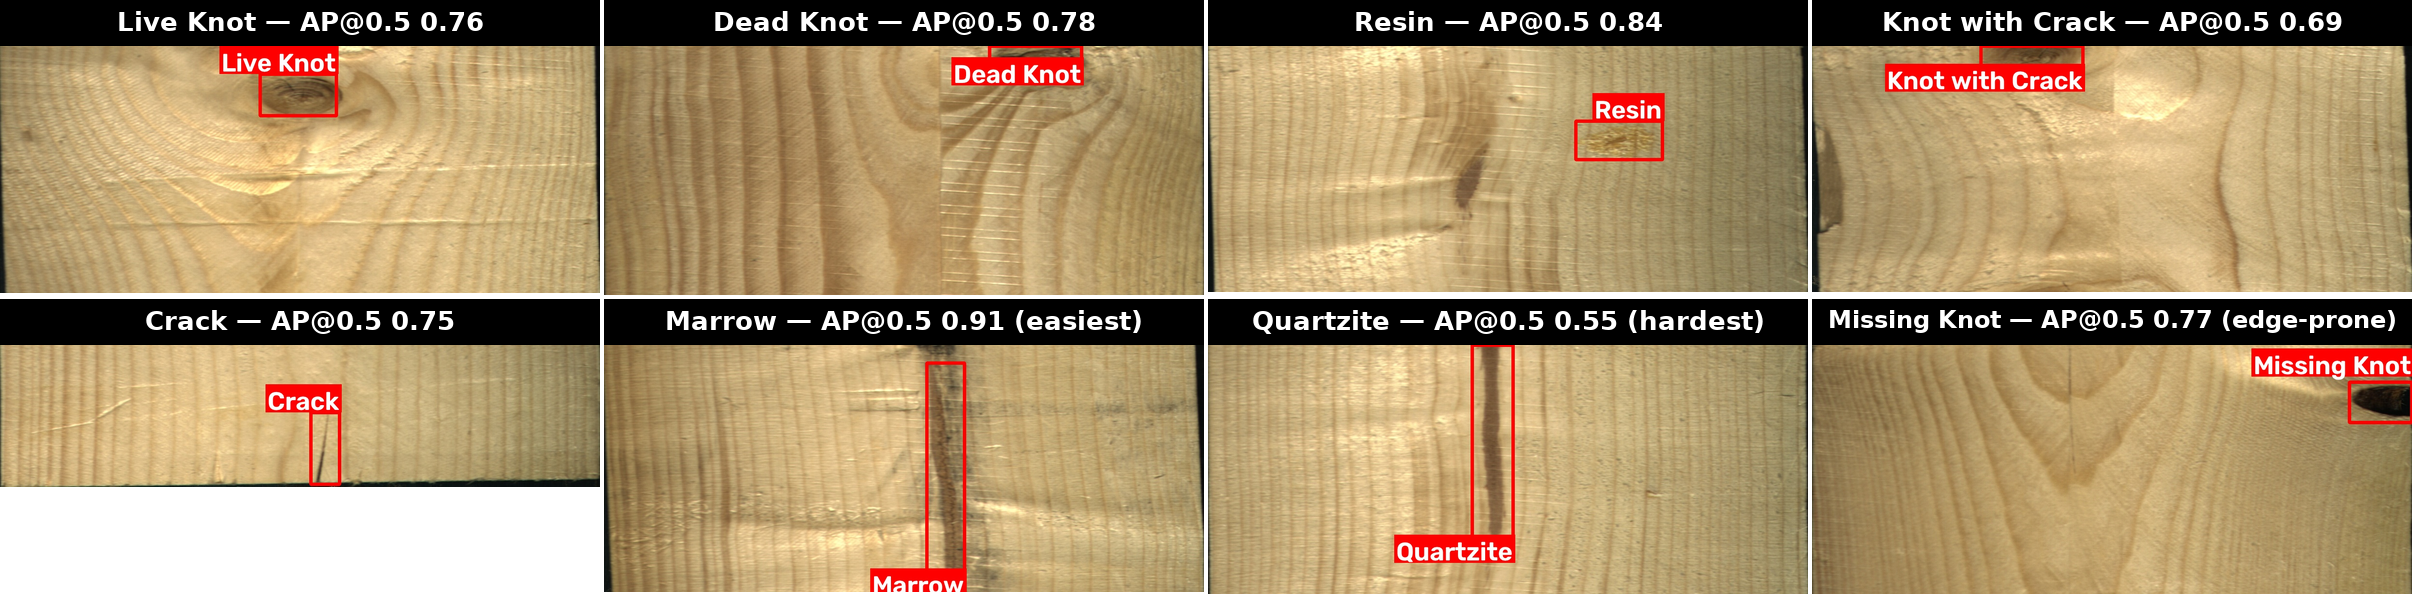
\includegraphics[width=\textwidth]{figures/results/inference_panel.png}
\caption{Ground-truth-annotated representative instances with best AP@0.5 per class.}
\label{fig:inference-panel}
\end{figure*}

Figure~\ref{fig:velocidad-precision} illustrates the trade-off between inference speed and precision. YOLO26 processes each image in 7.5~ms on average across the four configurations, RF-DETR in 12.6~ms, and Cascade R-CNN in 25.7~ms. Cascade R-CNN is 3.4 times slower than YOLO26 while its best mAP@0.5 of 0.677 trails RF-DETR's best of 0.717. RF-DETR offers the best ranking precision at 12.6~ms, 1.7 times slower than YOLO26, whose best mAP@0.5 is 0.618.

\begin{figure*}[t]
\centering
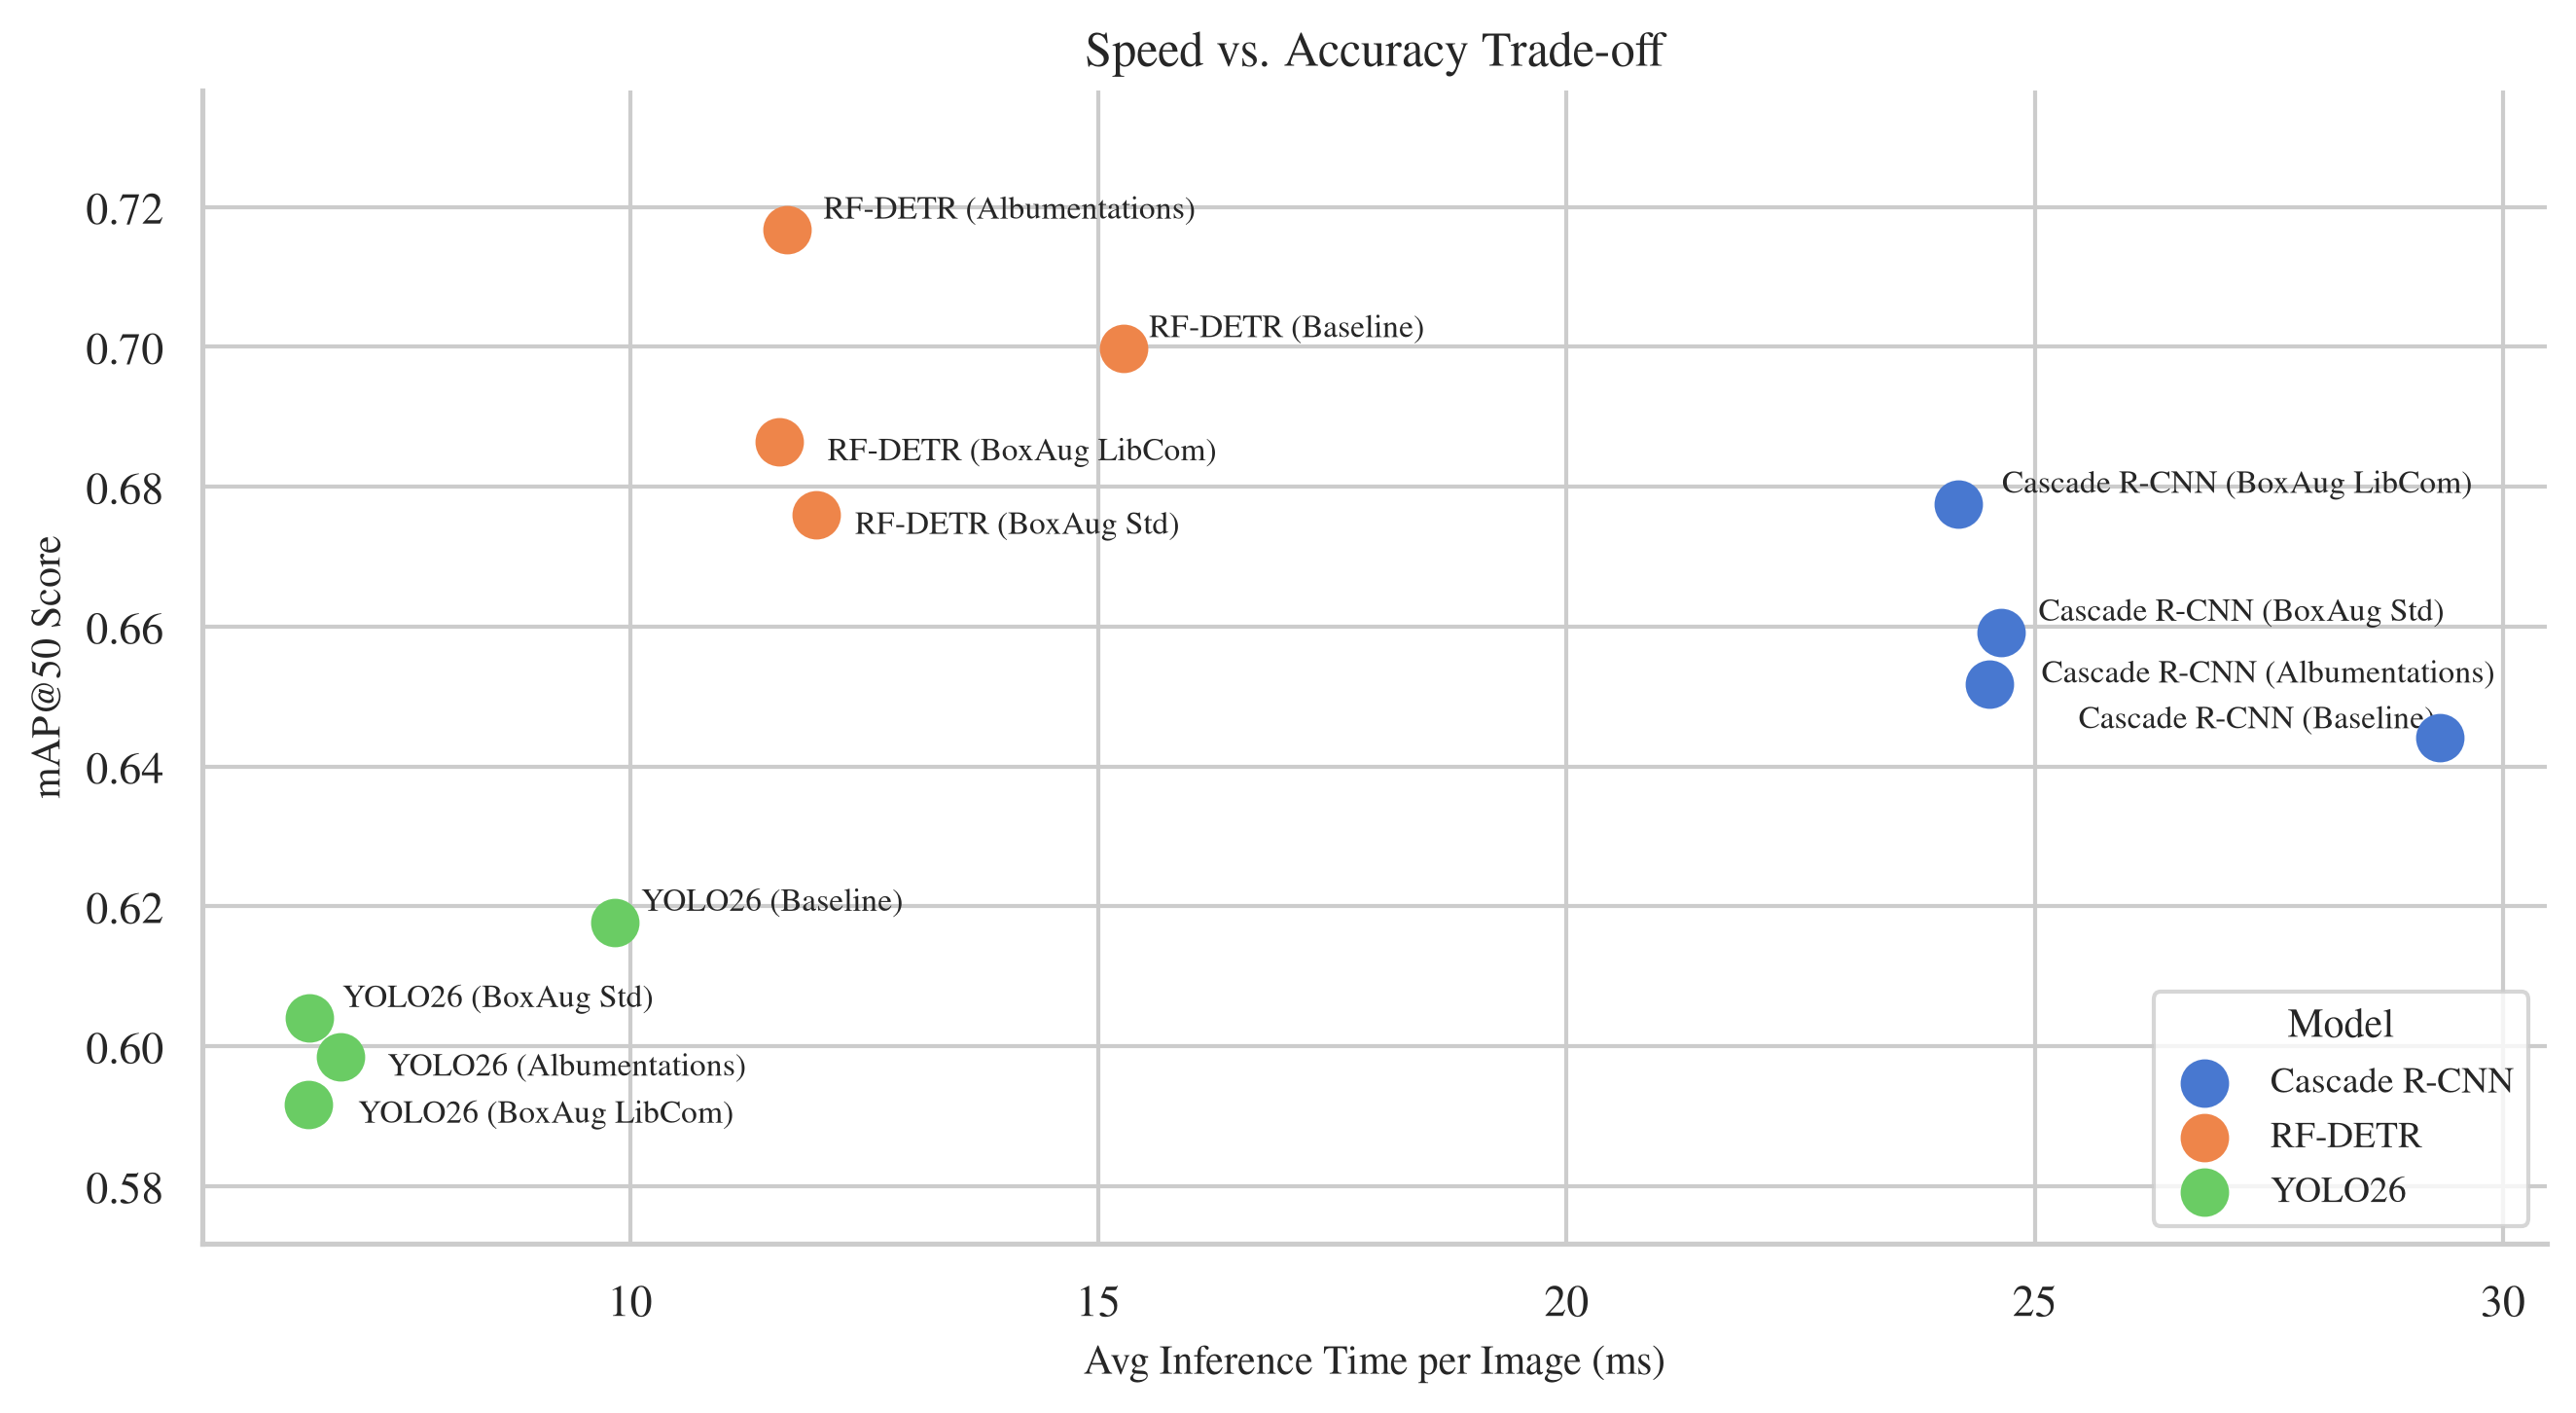
\includegraphics[width=\textwidth]{figures/results/speed_accuracy_tradeoff.png}
\caption{Trade-off between inference speed (ms/image) and precision (mAP@0.5).}
\label{fig:velocidad-precision}
\end{figure*}

Figure~\ref{fig:curvas-convergencia} shows the mAP@0.5 validation convergence curves throughout training epochs (Figure~\ref{fig:curvas-loss} shows the corresponding training losses). RF-DETR converges earliest, with best epoch between 6 and 11, Cascade R-CNN stabilizes between epoch 9 and 12 with BoxAug LibCom still climbing at epoch 12, and YOLO26 reaches its maximum between epochs 40 and 50, at the edge of its 50-epoch budget. YOLO26 curves show greater oscillation, particularly in the standard BoxAug configuration. This convergence pattern suggests that transformers need fewer iterations to capture relevant features, while one-stage convolutional architectures consume the full budget; the still-rising YOLO26 and Cascade LibCom curves indicate both budgets truncate learning. The oscillation in YOLO26 may indicate sensitivity to training sample variability in each batch.

\begin{figure*}[t]
\centering
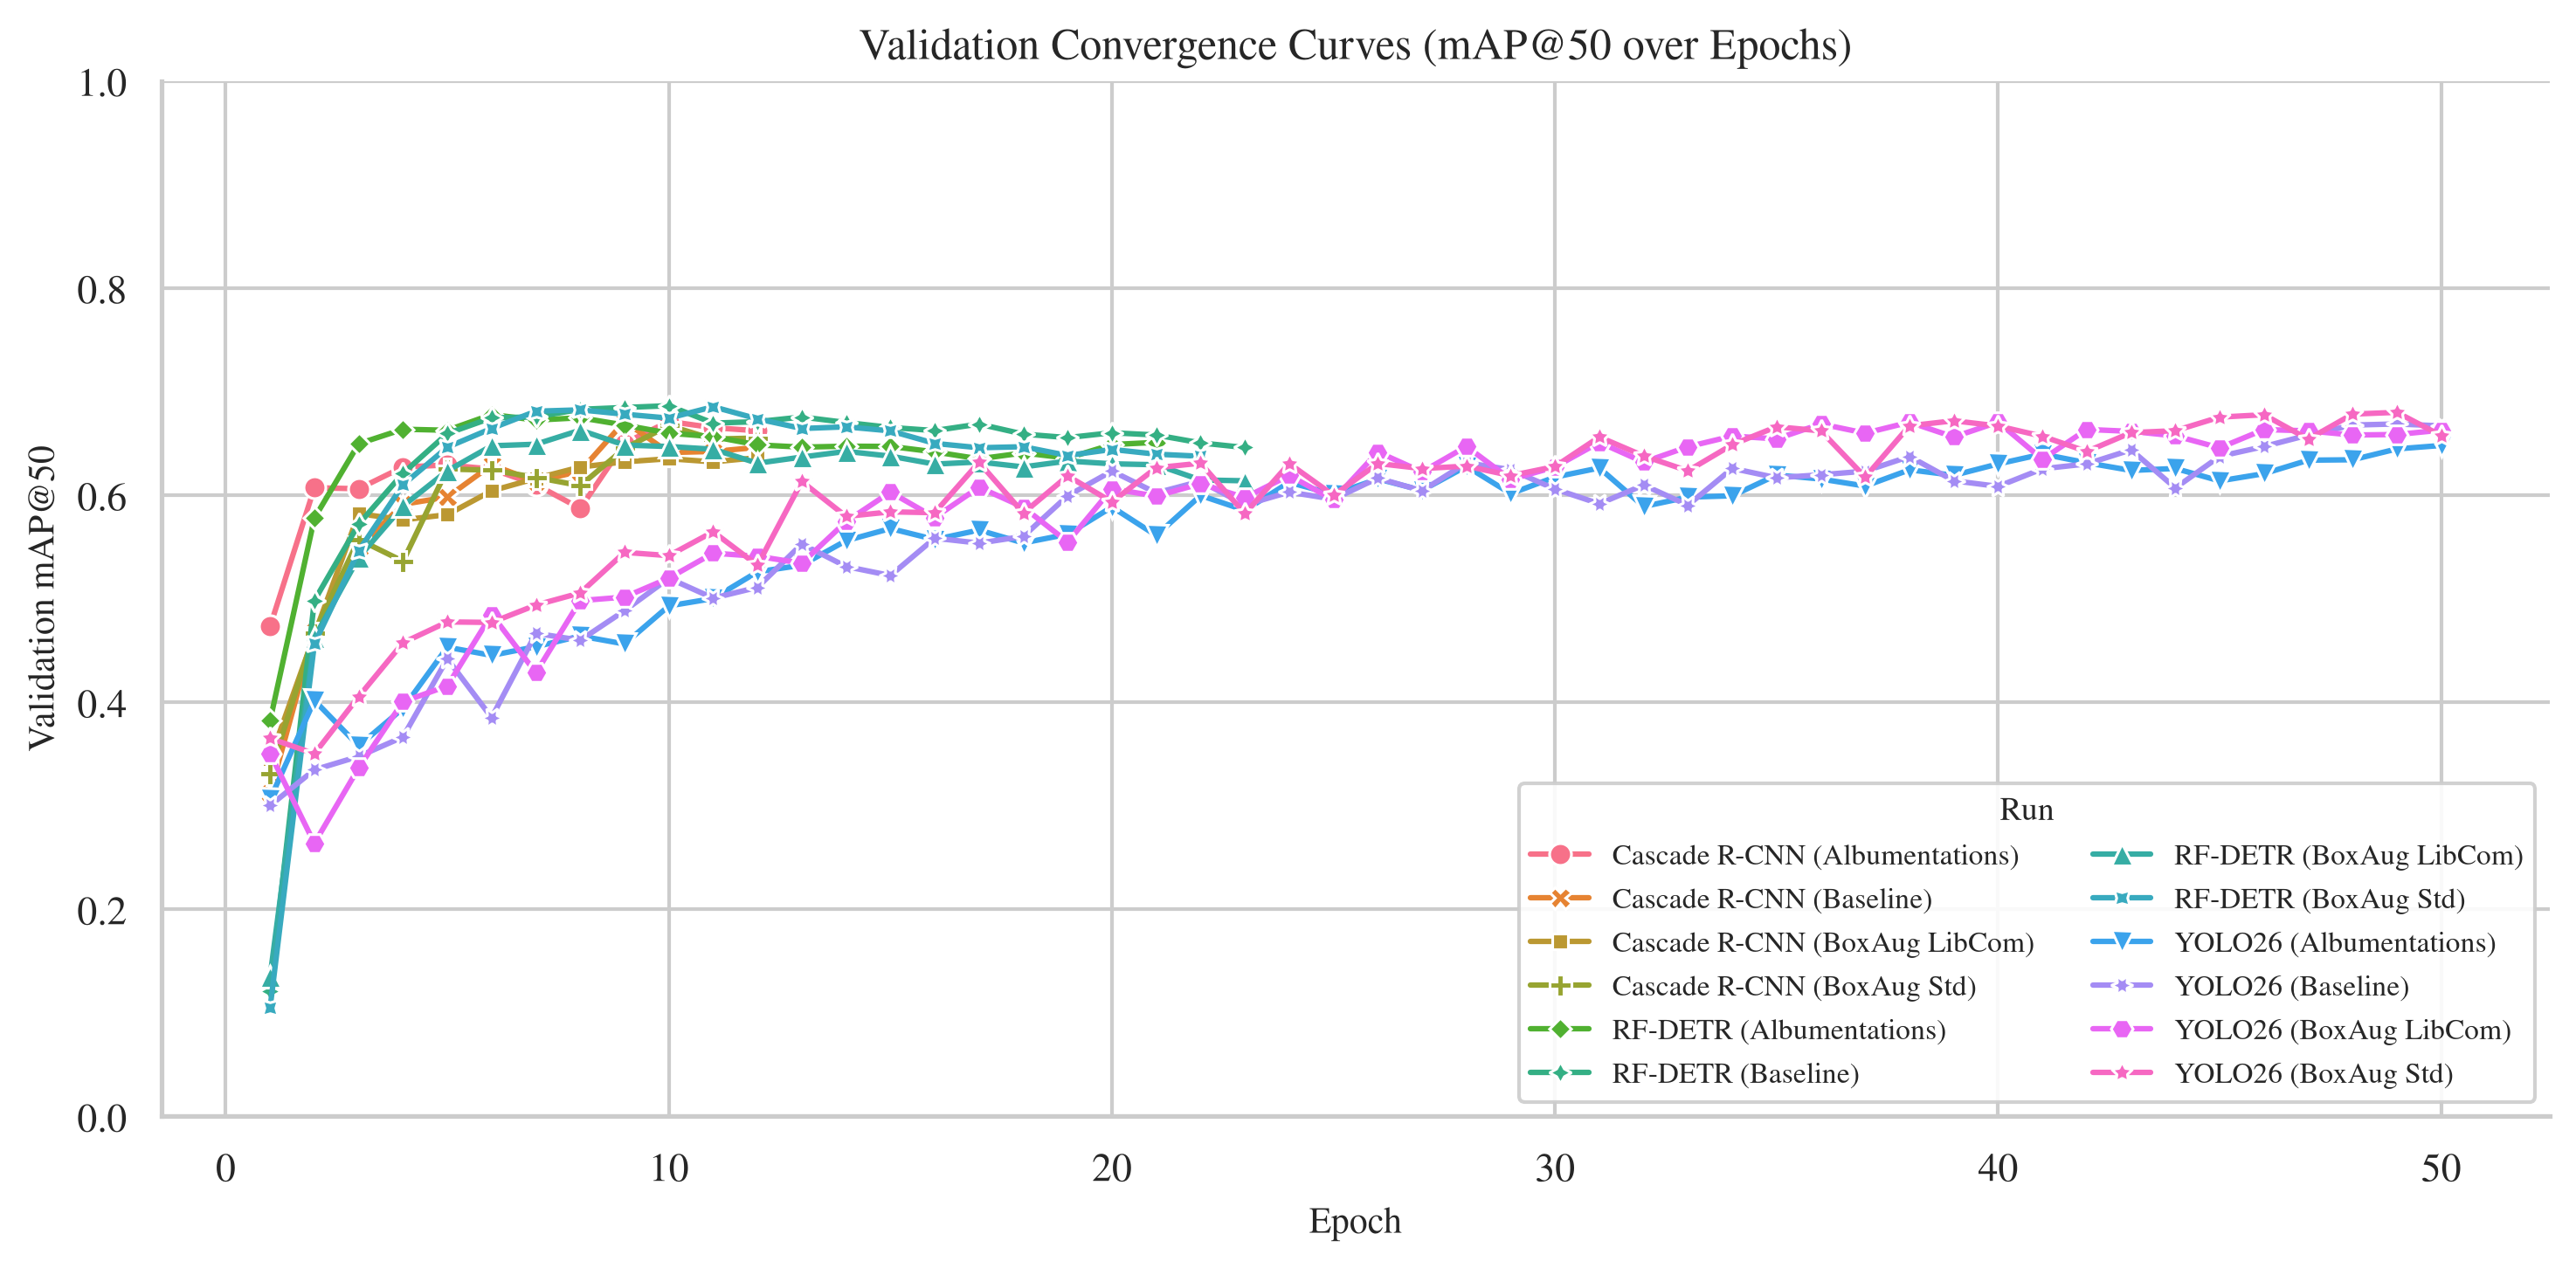
\includegraphics[width=\textwidth]{figures/results/training_curves_map.png}
\caption{mAP@0.5 validation convergence curves during training.}
\label{fig:curvas-convergencia}
\end{figure*}

\begin{figure*}[t]
\centering
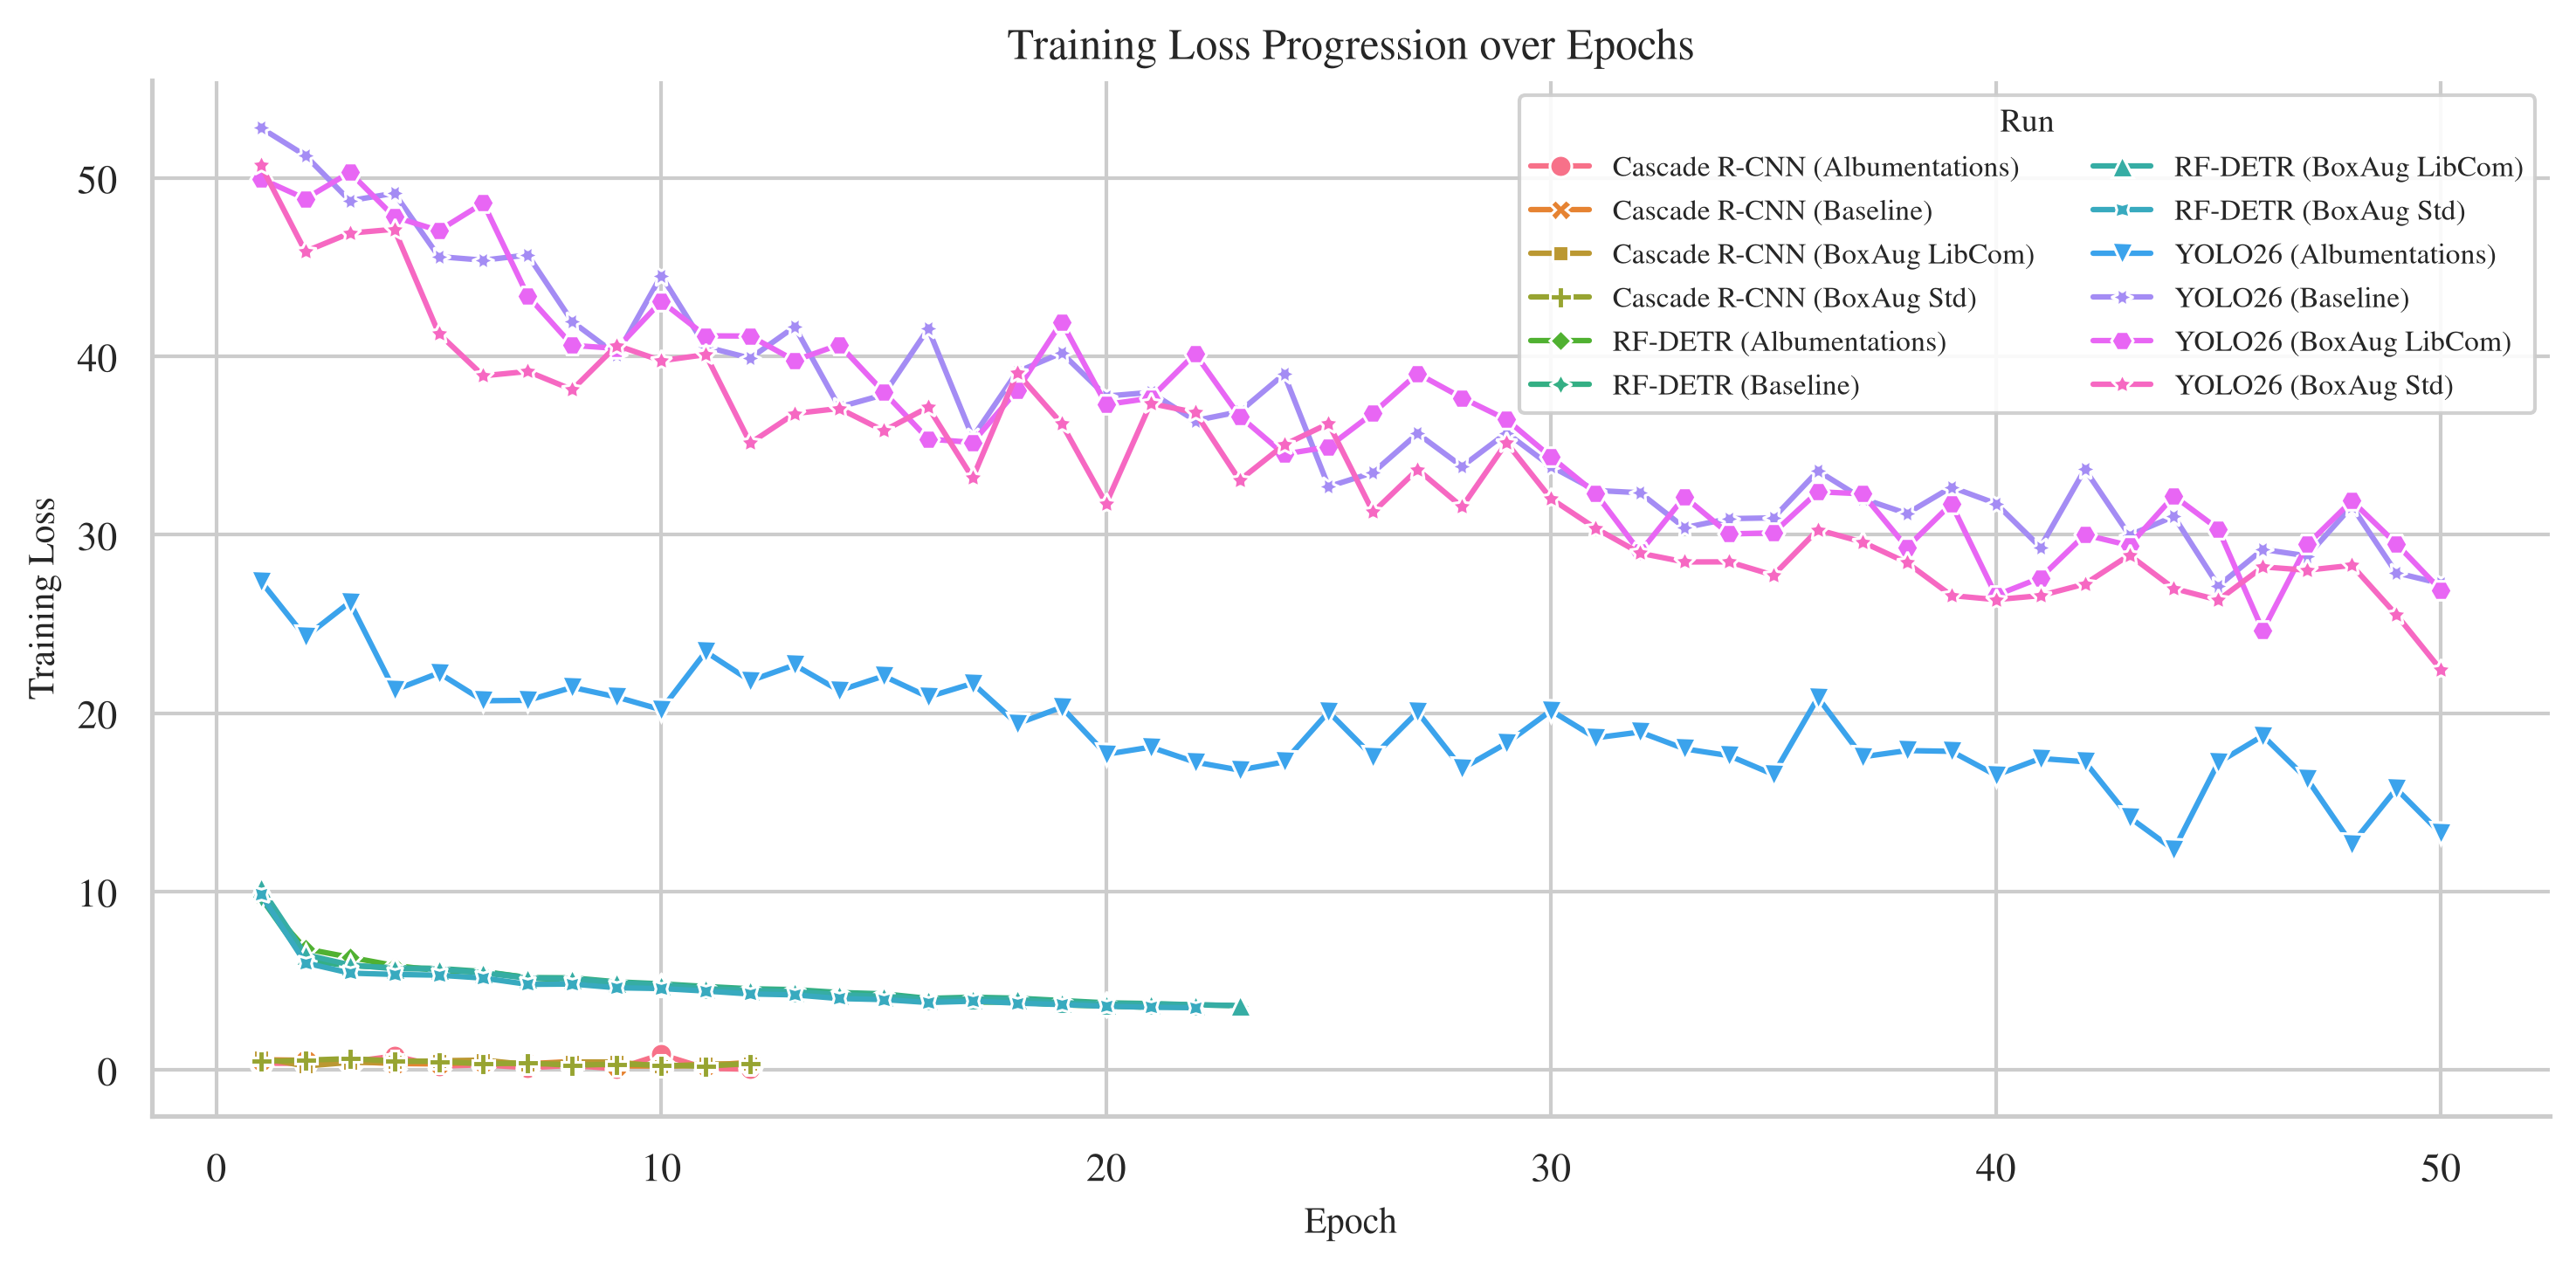
\includegraphics[width=\textwidth]{figures/results/training_curves_loss.png}
\caption{Training loss progression over epochs for all 12 configurations.}
\label{fig:curvas-loss}
\end{figure*}

Figure~\ref{fig:tiempo-entrenamiento} compares total training time per configuration. YOLO26 trains the full 50 epochs in 0.40 to 0.80 hours, Cascade R-CNN completes 12 epochs in 0.38 to 0.78 hours, and RF-DETR trains 21 to 23 epochs in 0.44 to 0.80 hours. Wall-clock budgets are therefore comparable across paradigms even though epoch counts differ, and per-epoch cost rather than early stopping dominates the differences.

\begin{figure*}[t]
\centering
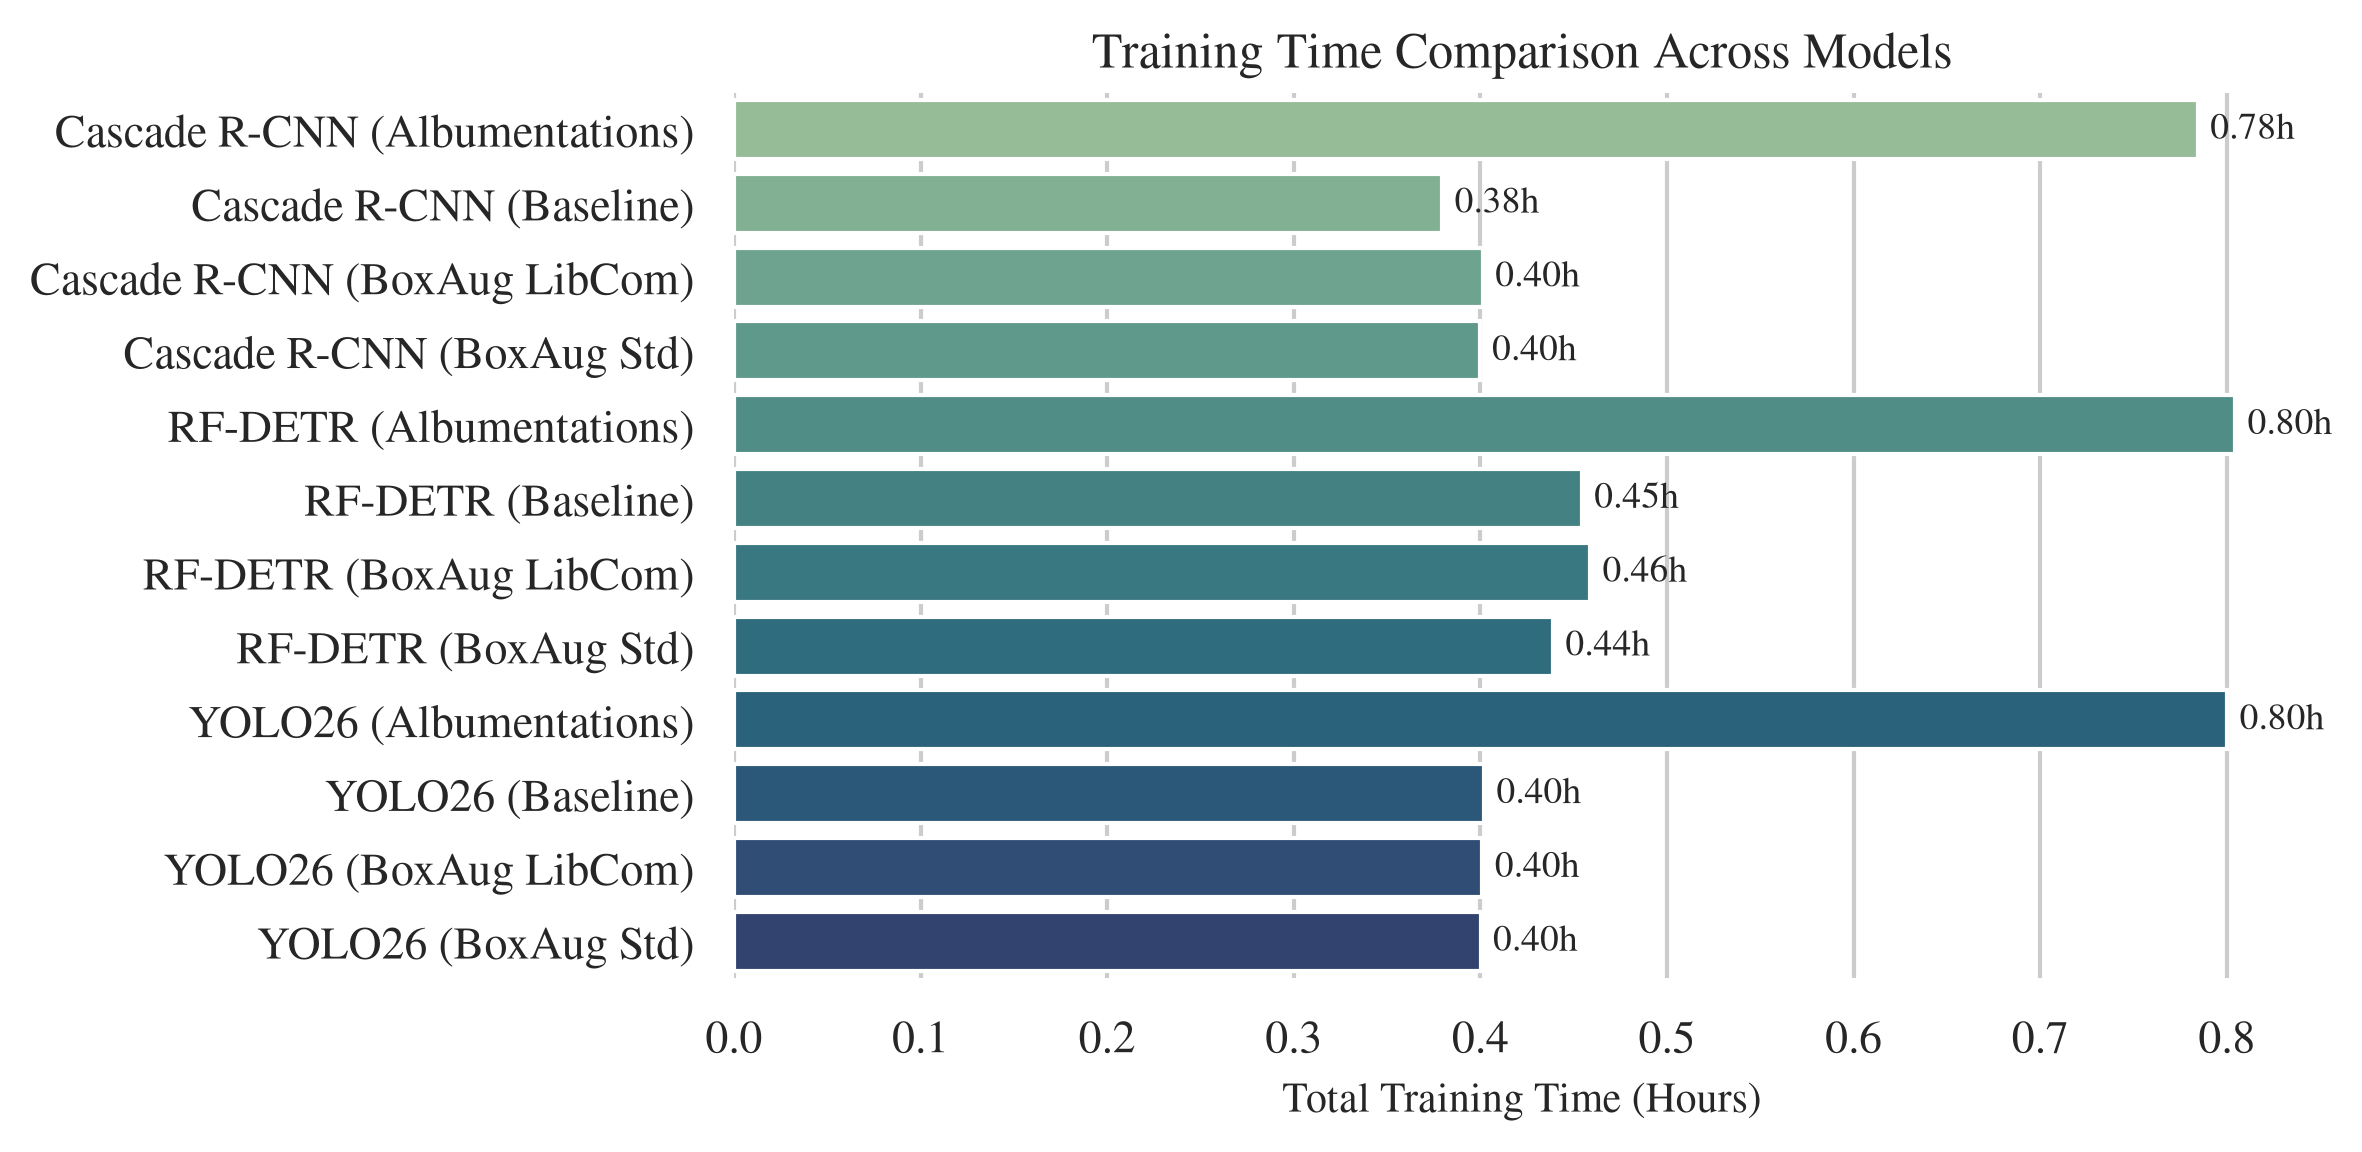
\includegraphics[width=\textwidth]{figures/results/training_time_comparison.png}
\caption{Comparison of total training time per configuration.}
\label{fig:tiempo-entrenamiento}
\end{figure*}

%% ============================================================
%% 5. DISCUSSION
%% ============================================================

\section{Discussion}
\label{sec:discussion}

The results obtained in this benchmark reveal patterns that warrant detailed analysis of the interactions between detection architectures and data augmentation strategies in the context of severe class imbalance typical of industrial wood inspection. RF-DETR's bidirectional global self-attention captures long-range spatial dependencies across the plank surface \cite{zhao2023detrs}. Cascade R-CNN remains the operating-point precision leader, with precision of 0.811 and F1 of 0.798 under BoxAug LibCom, consistent with cascaded refinement minimizing false positives through detection heads with increasing IoU thresholds \cite{cai2018cascade}. Notably, Cascade is the only paradigm that benefits from every augmentation strategy (+0.008 to +0.033), suggesting two-stage heads exploit synthetic minority instances once the operating point is fixed.

YOLO26 shows no augmentation dividend, the unaugmented baseline at mAP@0.5 of 0.618 beats all three augmented arms, which score 0.592 to 0.604. This contradicts the common expectation that one-stage detectors are the primary beneficiaries of training data volume \cite{hussain2023yolo}, at least under rectangular training with a full 50-epoch budget. A plausible mechanism is that YOLO26's anchor-free dense predictions already saturate on the majority distribution, so pasted minority instances add noise rather than signal at this budget. The greater oscillation observed in YOLO26 convergence curves, particularly in the standard BoxAug configuration, may be attributed to variability introduced by synthetic samples in a model that lacks Cascade R-CNN's multi-stage refinement mechanism. This result suggests that object augmentation techniques require larger budgets or cleaner synthesis to help one-stage detectors in severe imbalance scenarios. Naively pasted masks create pixel artifacts that detectors learn as shortcuts instead of appearance \cite{dwibedi2017cutpaste}; pasted small objects measurably degrade performance through overfitting to pasting artifacts such as imperfect masks and brightness mismatch \cite{kisantal2019small}, and context-agnostic pasting yields disharmonious, low-benefit samples \cite{guo2024cacp}. The YOLO family recipe itself excludes copy-paste (Mosaic/CutMix instead, copy-paste off by default and confined to segmentation tasks), so the null dividend is consistent with the architecture's design rather than a protocol bug. No published copy-paste ablation on YOLO26 exists to our knowledge; the cited drops are the closest measured analogues.

RF-DETR shows mixed behavior: Albumentations improves performance by +0.017, but standard BoxAug degrades it by -0.024 and BoxAug LibCom by -0.013. This result is particularly relevant for the research community in transformers for industrial vision \cite{hutten2022vision}. Patch-level noise transformations introduce artifacts that bidirectional global self-attention mechanisms interpret as relevant patterns, generating confusion during training. Unlike convolutional models that process local information through sliding filters, transformers capture long-range spatial dependencies that can amplify the influence of local artifacts \cite{zhao2023detrs}. The mechanism is structural. Standard BoxAug pastes patches with pixel-level noise and morphological perturbations \cite{LEE2022104138}, producing sharp edge gradients and high-frequency textures that do not occur in natural wood grain. During tokenization these discontinuities become outlier tokens; because every self-attention head computes Query-Key affinities over the full token set, a single anomalous patch can attract attention mass from distant, defect-free regions and propagate spurious correlations across layers. Convolutional detectors attenuate this effect through locality: sliding filters confine the artifact's receptive field, and Cascade R-CNN's staged IoU heads can still reject the proposal. Transformers have no such locality bottleneck, so the same artifact is broadcast globally. Neural harmonization via LibCom \cite{niu2021making} attenuates edge gradients through pixel-level color equalization \cite{Guerreiro_2023_CVPR}, which explains why BoxAug LibCom degrades RF-DETR less ($-$0.013) than the standard variant ($-$0.024): the pasted tokens remain distributionally closer to natural grain. The deflated-score phenomenon, where the same checkpoints collapse at a fixed 0.50 cutoff while ranking quality is preserved, further shows that threshold-then-mAP evaluation is brittle to calibration shifts. This result suggests that object augmentation strategies require careful adaptation when applied to self-attention-based architectures, and that operating points must be tuned per model rather than fixed globally. This asymmetry matches copy-paste's reported limits: it succeeds on two-stage detectors with long schedules, while strong augmentation can cost up to 1 AP point elsewhere \cite{ghiasi2021simple}.

Per-class analysis reveals counterintuitive results that challenge the assumption that class frequency directly determines detection difficulty. Quartzite, with only 144 annotations (1.6\% of the dataset), obtains the worst performance with AP@0.5 between 0.082 and 0.550, which is expected given its low visual contrast against wood grain. However, Marrow, with only 204 annotations, obtains the highest AP of up to 0.910. This disparity indicates that defect visual distinguishability is a determining factor that interacts with class frequency. Defects with distinctive visual patterns, such as marrow with its characteristic central line appearance, are more susceptible to automatic detection regardless of their representation in the dataset \cite{Chen2023Recognition}. Long-tail methods fail when they address only imbalance and ignore subtle inter-class differences \cite{zhang2021deep}, and raw counts overstate information because of overlap with diminishing returns \cite{cui2019classbalanced}. Marrow's high-contrast vertical central line gives a strong spatial signal-to-noise ratio learnable from few samples, while Quartzite shares reflectance and color with healthy grain: a camouflage regime where foreground-background similarity dominates difficulty \cite{fan2020cod} and natural texture variation masks the defect signal \cite{Chen2023Recognition}. Tail suppression by inter-class negative gradients \cite{tan2020equalization} then sinks the low-contrast class while sparing the distinctive one: detectability follows spatial SNR, not instance count.

Live Knot and Dead Knot, which together represent roughly 77\% of the dataset, show AP@0.5 values of 0.651 to 0.781 despite their high prevalence. This finding confirms that the high intra-class variance of these defects, where the same anomaly type can exhibit very different visual appearances \cite{Kodytek2022Dataset}, constitutes a challenge that is not resolved solely with greater data volume. Variability in the background wood grain, combined with different presentations of Live Knot and Dead Knot, generates a feature distribution that hinders model convergence toward robust discriminative representations. The 35\% majority downsampling of training planks combined with effective-number class weighting \cite{cui2019classbalanced} keeps minority classes competitive: the top configuration scores no class below 0.55. Loss-level treatments beyond a single fixed weighting, such as Focal Loss \cite{lin2017focal} or Seesaw Loss \cite{wang2021seesaw}, remain untested and could offer a more comprehensive solution for severe class imbalance. The source dataset itself warns that limitless variability cannot be fully captured by any finite sample \cite{Kodytek2022Dataset}.

In terms of computational efficiency, the speed-precision trade-off manifests differentially across the three paradigms. YOLO26 offers the best speed at 7.5~ms per image with mAP@0.5 of 0.618, which is relevant for high-throughput production lines \cite{Kodytek2022Dataset}. Cascade R-CNN is preferred when operating-point precision is prioritized over latency, reaching precision of 0.811 at 25.7~ms per image. RF-DETR offers the best ranking precision at 12.6~ms and mAP@0.5 of 0.717, positioning itself as a viable alternative for applications where the speed-precision trade-off must be balanced with the ability to capture long-range spatial dependencies. The selection of the optimal architecture will depend on the specific requirements of the industrial application, considering factors such as production line speed, false positive tolerance, and available computational resources. Selecting the architecture by speed/memory/accuracy balance for the target platform is the established practice \cite{huang2017speedaccuracy}; YOLO's real-time edge compatibility \cite{hussain2023yolo} versus DETR's NMS-free Pareto gains \cite{zhao2023detrs} frame the three operating points below.

%% ============================================================
%% 6. CONCLUSIONS
%% ============================================================

\section{Conclusions}
\label{sec:conclusions}

This study presented a comparative benchmark of three object detection paradigms with four data augmentation strategies for surface defect recognition in wood, evaluating 12 configurations on a dataset with severe imbalance of 1 to 35.3. The main results demonstrate that RF-DETR achieves the highest ranking precision with mAP@0.5 of 0.717 under per-model calibrated thresholds, Cascade R-CNN gains the most from augmentation with BoxAug LibCom contributing +0.033 and the best operating-point F1 of 0.798, and YOLO26 shows no augmentation dividend with its unaugmented baseline of 0.618 leading the family. Per-class analysis at AP@0.5 reveals that detection difficulty depends on both frequency and visual distinguishability of the defect, and the AP@0.5:0.95 view confirms this ordering while exposing weaker localization on the high-variance knot classes. Fixed confidence cutoffs mismeasure rect-trained models, so operating-point calibration is part of the method rather than an afterthought.

For deployment, the three paradigms occupy distinct operating points: YOLO26 at 7.5~ms per image suits high-throughput lines approaching 9.6~m/s where latency dominates; RF-DETR at 12.6~ms offers the best ranking precision for balanced speed--accuracy requirements; and Cascade R-CNN at 25.7~ms maximizes operating-point precision (0.811) where false positives are costly. These claims are bounded by the study's limits: single-run mAP point estimates without training variance, truncated epoch budgets that make the YOLO26 and Cascade LibCom scores lower bounds rather than converged values, and evaluation on a single species and industrial setup. The calibrated-threshold protocol, the paradigm-dependent augmentation response, and the released reproducible pipeline provide the baseline against which extended budgets, repeated runs with confidence intervals, and diffusion-based augmentation should be measured. Concretely: if the absolute priority is real-time speed to avoid production-line bottlenecks, choose YOLO26 (7.5~ms) \cite{hussain2023yolo,Kodytek2022Dataset}; for maximum defect-ranking precision in rigorous quality audit, choose RF-DETR (12.6~ms) \cite{zhao2023detrs}; and if a false positive carries severe economic loss, operate Cascade R-CNN with BoxAug LibCom (operating precision 0.811) \cite{cai2018cascade}.

%% ============================================================
%% 7. LIMITATIONS AND FUTURE WORK
%% ============================================================

\section{Limitations and Future Work}
\label{sec:future}

The fixed per-family epoch budgets truncate learning where curves still rise: YOLO26 best epochs fall between 40 and 50 of a 50-epoch budget, and Cascade R-CNN with BoxAug LibCom is still climbing at epoch 12 of 12, so reported scores are lower bounds for those configurations rather than converged values. Extending YOLO26 beyond 50 epochs and Cascade R-CNN to its 2x schedule would test whether the ranking holds at convergence. All mAP values reported are single-run point estimates; a three-seed repeat protocol (seeds 42--44, mean $\pm$ std) is the natural next step for training-variance intervals around mAP. The most immediate modeling direction corresponds to diffusion-based augmentation. The cut-and-paste methods evaluated, such as BoxAug, are limited by the number of rare instances available for cropping from the original dataset. With only 144 quartzite annotations, the object bank is too small to generate diverse augmentation. Conditional diffusion models such as Stable Diffusion with ControlNet can generate synthetic instances of rare classes without relying on existing crops, offering a potentially more effective alternative for severe imbalance \cite{capogrosso2024diffusion}.

The per-class AP heatmaps above remain point estimates (the Bonferroni-binomial construction does not apply to AP, a ranking metric), and cross-class confusion is folded into per-class false positives and false negatives rather than shown as an off-diagonal matrix.

Expanding the dataset to other wood species with different grain patterns and defects is essential to validate generalization beyond the current species and industrial environment. In parallel, model quantization to INT8 and FP16 could reduce inference times for deployment on production lines with hardware constraints, while evaluating transformer architectures such as DINO and Grounding DINO could determine whether global self-attention mechanisms improve detection of low-contrast defects. The combination of multiple research directions, including class weighting, diffusion-based augmentation, and model optimization, could lead to more robust and efficient inspection systems for the wood industry. These future directions seek to address the limitations identified in the present benchmark and bring automated detection systems closer to the operational requirements of wood processing plants. The development of reproducible experimental pipelines, such as the one employed in this study, will facilitate comparative evaluation of new techniques emerging from these research directions.

\FloatBarrier

%% ============================================================
%% DECLARATIONS
%% ============================================================

\section*{CRediT authorship contribution statement}
\textbf{Ricardo Mauricio Chambilla Perca:} Software, Writing - Original Draft. \textbf{Mariel Alison Jara Mamani:} Data Curation, Resources, Methodology. \textbf{Christian Raul Mestas Zegarra:} Project administration, Conceptualization, Writing - Review \& Editing. \textbf{Yenaro Joel Noa Camino:} Investigation, Resources. \textbf{Luis Gustavo Sequeiros Condori:} Conceptualization, Investigation, Software. \textbf{Yasiel P\'erez Vera:} Supervision, Writing - Review \& Editing.

\section*{Conflict of Interest Declaration}
The authors declare that they have no known competing financial interests or personal relationships that could have appeared to influence the work reported in this article.

\section*{Code Availability}
Custom analysis scripts and source code generated during this study are publicly available at the GitHub repository: \url{https://github.com/christianmz565/ia-2026-final}, licensed under the AGPL-3.0 license.

\section*{Data Availability}
The data used in this study are publicly available on Kaggle: \url{https://www.kaggle.com/datasets/nomihsa965/large-scale-image-dataset-of-wood-surface-defects}, licensed under the CC BY 4.0 license.

\FloatBarrier

%% ============================================================
%% REFERENCES
%% ============================================================

\bibliographystyle{elsarticle-num}
\bibliography{references}

\end{document}
